% v2-acmsmall-sample.tex, dated March 6 2012
% This is a sample file for ACM small trim journals
%
% Compilation using 'acmsmall.cls' - version 1.3 (March 2012), Aptara Inc.
% (c) 2010 Association for Computing Machinery (ACM)
%
% Questions/Suggestions/Feedback should be addressed to => "acmtexsupport@aptaracorp.com".
% Users can also go through the FAQs available on the journal's submission webpage.
%
% Steps to compile: latex, bibtex, latex latex
%
% For tracking purposes => this is v1.3 - March 2012

\documentclass[prodmode,acmtodaes]{acmsmall} % Aptara syntax

% Package to generate and customize Algorithm as per ACM style
\usepackage[ruled,linesnumbered]{algorithm2e}
\renewcommand{\algorithmcfname}{ALGORITHM}
\SetAlFnt{\small}
\SetAlCapFnt{\small}
\SetAlCapNameFnt{\small}
\SetAlCapHSkip{0pt}
\IncMargin{-\parindent}

% Metadata Information
\acmVolume{9}
\acmNumber{4}
\acmArticle{39}
\acmYear{2010}
\acmMonth{3}

% Document starts
\begin{document}

% Page heads
\markboth{Y. Qin et al.}{Complementary Synthesis for Encoder with Flow Control Mechanism}

% Title portion
\title{Complementary Synthesis for Encoder with Flow Control Mechanism}
\author{YING QIN and
SHENGYU SHEN and
QINGBO WU and
HUADONG DAI and
YAN JIA  
\affil{School of Computer, National University of Defense Technology}}
% NOTE! Affiliations placed here should be for the institution where the
%       BULK of the research was done. If the author has gone to a new
%       institution, before publication, the (above) affiliation should NOT be changed.
%       The authors 'current' address may be given in the "Author's addresses:" block (below).
%       So for example, Mr. Abdelzaher, the bulk of the research was done at UIUC, and he is
%       currently affiliated with NASA.

\begin{abstract}
Complementary synthesis automatically generates an encoder's decoder
with the assumption that the encoder's all input variables can always 
be uniquely determined by its output symbol sequence.
However,
to prevent the faster encoder from overwhelming the slower decoder,
many encoder employ flow control mechanism that fails this assumption.
Such encoders,
when its output symbol sequence is too fast to be processed by the decoder,
will stop transmitting data symbols,
but instead transmitting an idle symbol that can only uniquely determine a subset of the encoder's input variables.
And the decoder should recognize and discard this idle symbol.
Although this mechanism can prevent losing data symbols,
it fails the assumption of all complementary synthesis algorithms,
because some input variables can not be uniquely determined by the idle symbol.

This paper proposes the first algorithm 
to handle such encoders.
\textbf{First},
it identifies all input variables that can be uniquely determined,
and take them as flow control variables.
\textbf{Second},
it infers a predicate over these flow control variables,
that enables all other input variables to be uniquely determined.
\textbf{Third},
the decoder's Boolean function for flow control variables can be characterized with Craig interpolant.
For other input variables,
their decoder's Boolean function can also be characterized similarly but the inferred predicate must be enforced first.

Experimental results on several complex encoders indicate that
our algorithm can always correctly identify the flow control variables,
infer the predicates
and generate the decoder's Boolean functions.
\end{abstract}

\category{B.5.2}{Design Aids}{Automatic synthesis}
\category{B.6.3}{Design Aids}{Automatic synthesis}

\terms{Algorithms, Logic synthesis, Verification}

\keywords{Craig interpolation, decoder, encoder, finite-state transition system, satisfiability solving}

\acmformat{Ying Qin and
ShengYu Shen and
QingBo Wu and
HuaDong Dai and
Yan Jia, 2014. Complementary Synthesis for Encoder with Flow Control Mechanism.
% ACM Trans. Embedd. Comput. Syst. X, X, Article XX (XXXX 201X), X pages.
% DOI:http://dx.doi.org/10.1145/0000000.0000000
}
% At a minimum you need to supply the author names, year and a title.
% IMPORTANT:
% Full first names whenever they are known, surname last, followed by a period.
% In the case of two authors, 'and' is placed between them.
% In the case of three or more authors, the serial comma is used, that is, all author names
% except the last one but including the penultimate author's name are followed by a comma,
% and then 'and' is placed before the final author's name.
% If only first and middle initials are known, then each initial
% is followed by a period and they are separated by a space.
% The remaining information (journal title, volume, article number, date, etc.) is 'auto-generated'.

\begin{bottomstuff}
This work was funded by projects 61070132 and 61133007 supported by National Natural Science Foundation of China,
the 863 Project of China under contract 2012AA01A301.

Author's addresses: Ying Qin,
ShengYu Shen,
QingBo Wu,
HuaDong Dai and 
Yan Jia , School of Computer, National University of Defense Technology.
\end{bottomstuff}
\markboth{Ying Qin et al.}{Complementary Synthesis for Encoder with Flow Control Mechanism}

\maketitle


\section{Introduction}

One of the most difficult jobs in designing communication
and multimedia chips is to design and verify complex encoder and decoder pairs.
The encoder maps its input variables $\vec{i}$ to its output variables $\vec{o}$,
% according to some predefined rules,
% such as Ethernet \cite{IEEE8023_S4} and PCI Express \cite{pcie21},
while the decoder recovers $\vec{i}$ from $\vec{o}$.
\textbf{
Complementary synthesis [\citeNP{ShenICCAD09};\citeyearNP{ShenTCAD10,ShenTCAD11,ShenTCAD12};\citeNP{LiuICCAD11};\citeyearNP{LiuTCAD12};\citeNP{TuDAC13}]
try to ease this job by
automatically generating a decoder from an encoder's specification,
with the assumption that $\vec{i}$ can always be
uniquely determined by a bounded sequence of $\vec{o}$.}

\textbf{
However, 
the encoders of many high speed communication systems employ flow control mechanism \cite{flowcontrol} that 
fails this assumption.
Figure~\ref{fig:nonuniq}a) shows such a communication system with flow control mechanism,
which include a faster transmitter and a slower receiver connected by a pair of encoder and decoder.
There are two input variables from the transmitter to the encoder:
the data bit $d$ to be encoded,
and the flow control bit $f$ indicating the validness of $d$.
Figure~\ref{fig:nonuniq}b) shows the mapping table of the encoder
that maps $f$ and $d$ to the output symbol $\vec{o}$.
% It is obvious that,
% when $f\equiv 1$,
% by checking whether $o$ is $D_0$ or $D_1$,
% we can determine whether the $d$ is 0 or 1;
% But when $f\equiv 0$,
% we can not determine the value of $d$,
% because $o$ is always $I$.
}

\textbf{
The flow control mechanism prevent the faster transmitter from overwhelming the slower receiver in the following way:
\begin{enumerate}
\item
When the receiver can keep up with the transmitter,
the transmitter will rise $f$ to 1, 
which makes the encoder to transmit $D_d$ according to the value of $d$.
And the decoder can always recover both $f$ and $d$ from $D_d$ according to Figure~\ref{fig:nonuniq}b).
\item
But when the receiver can not keep up with the transmitter,
the transmitter will drop $f$ to 0 to stop the encoder transmitting new $D_d$,
but instead transmitting the idle symbol $I$ without considering the value of $d$.
And the decoder should discard this idle symbol $I$,
and send $f\equiv 0$ to the receiver with whatever value on $d$.
\end{enumerate}
}

\textbf{
This mechanism can prevent the faster transmitter from transmitting too much data 
that can not be handled by the slower receiver.
But it fails the assumption of all current complementary synthesis algorithms 
[\citeNP{ShenICCAD09};\citeyearNP{ShenTCAD10,ShenTCAD11,ShenTCAD12};\citeNP{LiuICCAD11};\citeyearNP{LiuTCAD12};\citeNP{TuDAC13}],
because $d$ can not be uniquely by the idle symbol $I$.
It is obvious that,
to resolve this issue and generate the decoder,
we only need to consider the case $f\equiv 1$,
in which $d$ can be uniquely determined.
For other cases in which $f\equiv 0$,
$d$ is not need by the receiver and can be any value.}

\begin{figure}
\centerline{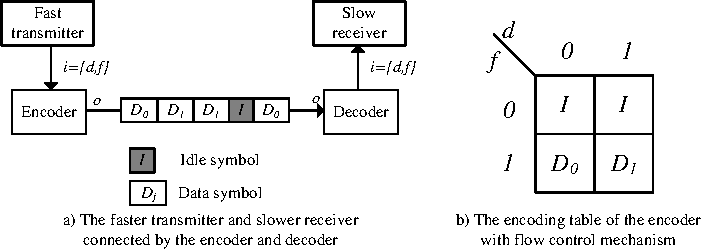
\includegraphics[width=\textwidth]{nonuniq}}
\caption{An encoder with flow control mechanism}
\label{fig:nonuniq}
\end{figure}


Thus,
according to this insight,
we propose in this paper the first complementary synthesis algorithm 
to handle encoders with flow control mechanism in three steps:
\textbf{First},
it applies the classical halting complementary synthesis algorithm \cite{ShenTCAD11}
to identify all the input variables of the encoder that can be uniquely determined,
and call them the flow control variables $\vec{f}$.
Other input variables that can not be uniquely determined is called the data variables $\vec{d}$.
\textbf{Second},
it infers a sufficient and necessary predicate $valid(\vec{f})$ that enables $\vec{d}$ to be uniquely determined
by a bounded sequence of the encoder's output variables $\vec{o}$.
\textbf{Finally},
% $\vec{f}$ can be uniquely determined by $\vec{o}$,
it characterizes the decoder's Boolean function that computes each flow control variable $f\in\vec{f}$ 
by building a Craig interpolant\cite{interp_McMillan}.
On the other hand,
for other data variables $\vec{d}$,
their values are meaningful only when $valid(\vec{f}) \equiv 1$.
Thus, the decoder's Boolean function of each $d\in\vec{d}$ can be built similarly with Craig interpolant,
but only after enforcing $valid(\vec{f}) \equiv 1$.

The second step of this algorithm seems somewhat similar to that of \cite{ShenTCAD12} in the sense that 
both algorithms infer predicates that enable $\vec{d}$ or $\vec{i}$ to be uniquely determined.
But the essential difference between them is that
the algorithm of \cite{ShenTCAD12} infers a global assertion 
that must be enforced on all steps along the unrolled state transition sequence,
% so that the encoder eventually reaches and never leaves the unique state set,
while our algorithm infers a local predicate that is only enforced 
at the current step when we need to recover the value of $\vec{d}$.
Thus,
our algorithm can be seen as a generalization of \cite{ShenTCAD12}.

% This new algorithm has been implemented with the OCaml language. 
% All generated SAT instances are solved with Minisat solver \cite{EXTSAT}. 
Experimental results indicate that,
for several complex encoders from real projects (e.g., Ethernet \cite{IEEE8023_S4} and PCI Express \cite{pcie21}),
our algorithms can always correctly identify the flow control variables, infer the predicates and generate the decoders. 
In addition,
we also conduct other experiments to compare our algorithms with the state-of-the-art complementary synthesis algorithms.
All these experimental results and programs can be downloaded from https://github.com/shengyushen/compsyn.


\emph{The remainder of this paper is organized as follows}.
%Section \ref{sec_casestudy} explains our ideas with a simple example.
Section \ref{sec_prem} introduces the background material;
Section \ref{sec_findfc} presents the algorithm that identifies the flow control variables,
while Section \ref{sec_infer} infers the predicate that enables $\vec{d}$ to be uniquely determined by a bounded sequence of $\vec{o}$;
Section \ref{sec_min} minimizes the length of unrolled state sequence,
while Section \ref{sec_char} presents the algorithm to characterize the decoder's Boolean function;
Sections \ref{sec_exp} and \ref{sec_relwork} present the experimental results and related works;
Finally,
Section \ref{sec_conclude} sums up the conclusion.

\section{Preliminaries}\label{sec_prem}

% \subsection{Flow control mechanism}\label{subsec_fc}



\subsection{Propositional satisfiability}\label{subsec_SAT}
% We use a denotation similar to that of \cite{TuDAC13}.
The Boolean value set is denoted as $B=\{0,1\}$.
A vector of variables is represented as $\vec{v}=(v,\dots)$.
The number of variables in $\vec{v}$ is denoted as $|\vec{v}|$.
If a variable $v$ is a member of $\vec{v}$,
% that is $\vec{v}=(\dots,v,\dots)$,
then we say $v\in\vec{v}$;
otherwise we say $v\notin\vec{v}$.
For a variable $v$ and a vector $\vec{v}$,
if $v\notin\vec{v}$,
then the new vector that contains both $v$ and all members of $\vec{v}$ is denoted as $v\cup\vec{v}$.
If $v\in \vec{v}$,
then the new vector that contains all members of $\vec{v}$ except $v$,
is denoted as $\vec{v}-v$.
For the two vectors $\vec{a}$ and $\vec{b}$,
the new vector with all members of $\vec{a}$ and $\vec{b}$ is denoted as $\vec{a}\cup\vec{b}$.
The set of truth valuations of $\vec{v}$ is denoted as $[\![\vec{v}]\!]$,
for instance,
$[\![(v_1,v_2)]\!]=\{(0,0),(0,1),(1,0),(1,1)\}$.

A Boolean formula $F$ over a variable set $V$ is constructed by connecting variables from $V$ 
with symbols $\neg$, $\wedge$, $\vee$ and $\Rightarrow$,
which stand for logical connectives negation, conjunction, disjunction, and implication, respectively.

The propositional satisfiability problem(abbreviated as SAT) for a Boolean formula $F$ over a variable set $V$ 
is to find a satisfying assignment $A:V\to B$,
so that $F$ can be evaluated to $1$.
If such a satisfying assignment exists, then $F$ is satisfiable;
otherwise,
it is unsatisfiable.

% A computer program that decides the existence of such a satisfying assignment is called a SAT solver,
%  such as Zchaff\cite{CHAFF},
%  Grasp\cite{grasp},
%  Berkmin\cite{BERKMIN},
%  and MiniSat\cite{EXTSAT}.
 
% Normally,
% a SAT solver requires the formula to be represented in the conjunctive normal form(CNF),
% in which a formula is a conjunction of its clause set,
% and a clause is a disjunction of its literal set,
% and a literal is a variable or its negation.
% A formula in the CNF format is also called a SAT instance,


% \subsection{Cofactoring}\label{subsec_pre_cofact}

% For a Boolean function $f:B^n\to B$,
% we use $supp(f)$ to denote its support set $\{v_1\dots v_n\}$.
According to \cite{EFFSATUSMCCO},
the positive and negative cofactors of $f(v_1\dots v\dots v_n)$ with respect to variable
$v$ are $f_{v\equiv 1}=f(v_1\dots 1\dots v_n)$ and $f_{v\equiv 0}=f(v_1\dots 0\dots v_n)$,
respectively.
% Existential quantification of $f(v_1\dots v\dots v_n)$ with respect to a
% variable $v$ is $\exists v f=f_v+f_v’$.
\textbf{Cofactoring} is the action that applies 1 or 0 to $v$ to get $f_{v\equiv 1}$ or $f_{v\equiv 0}$.

% \subsection{Craig interpolation}\label{subsec_pre_interp}
% Craig\cite{Craig} had proved the following theorem:
% \begin{theorem}[Craig Interpolation Theorem\cite{Craig}]\label{thm_craig}
Given two Boolean formulas $\phi_A$ and $\phi_B$,
with $\phi_A\wedge \phi_B$ unsatisfiable,
there exists a formula $\phi_I$ referring only
to the common variables of $\phi_A$ and $\phi_B$ such that $\phi_A\Rightarrow \phi_I$
and $\phi_I\wedge \phi_B$ is unsatisfiable.
We call $\phi_I$ the \textbf{interpolant}\cite{Craig} of $\phi_A$ with respect to $\phi_B$
% \end{theorem}
and use McMillan's algorithm \cite{interp_McMillan} to generate it.

% In the remainder of this paper,
% we will focus on the propositional logic only,
% There are many approaches to generate interpolants for propositional logic,
% so please refer to Krajicek\cite{interp_Krajicek},
% Pudlak\cite{interp_Pudlak} and McMillan\cite{interp_McMillan} for more details.
% which is generated by MiniSat\cite{EXTSAT}.


\subsection{Incremental SAT mechanism of MiniSat solver}\label{subsec_incsat}

In this paper,
we use the MiniSat solver \cite{EXTSAT} to solve the generated CNF formulas.
Like many other SAT solver based on conflict driven learning \cite{CONFLICTLEARN},
MiniSat generates learned clauses from conflicts in searching,
and records them to prevent the same conflict from rising again.
This mechanism can significantly speedup a particular SAT solving.

In many applications,
there often exists a serial of CNF formulas tightly related to each other.
If the learned clauses can be shared between them,
then these formulas can be solved much faster.

MiniSat provides an incremental SAT mechanism to reuse these learned clauses.
This mechanism includes two procedures:
\begin{enumerate}
\item
$addClause(F)$ used to add a CNF formula $F$ to the clause database of MiniSat.
\item
$solve(A)$ that takes a set of literals $A$ as assumptions,
and solves the CNF formula $F\wedge \bigwedge_{a\in A} a$.
\end{enumerate}


\subsection{Finite state machine}

% \begin{figure}[t]
% \centering
% 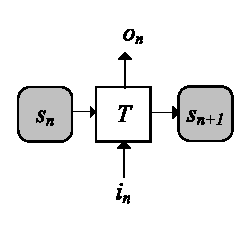
\includegraphics{mealy}
% \caption{Mealy finite state machine}
% \label{mealy}
% \end{figure}

The encoder is modeled by a finite state machine(FSM) $M=(\vec{s},\vec{i},\vec{o},T)$,
consisting of a state variable vector $\vec{s}$,
% an initial state $s_0\in S$,
an input variable vector $\vec{i}$,
% a finite set of configuration letters $C$,
an output variable vector $\vec{o}$,
and a transition function $T: [\![\vec{s}]\!]\times [\![\vec{i}]\!]\to [\![\vec{s}]\!]\times [\![\vec{o}]\!]$ 
that computes the next state and output variable vector from the current state and input variable vector.

% As shown in Figure \ref{mealy},
% as well as in the remainder of this paper,
% the state is represented as a gray round corner box,
% and the transition function $T$ is represented as a white rectangle.
The behavior of FSM $M$ can be reasoned by unrolling transition function for multiple steps.
The state variable $s\in\vec{s}$, input variable $i\in\vec{i}$ and output variable $o\in\vec{o}$ at the $n$-th step 
are respectively denoted as $s_n$, $i_n$ and $o_n$.
Furthermore,
the state, the input and the output variable vectors at the $n$-th step are respectively denoted as $\vec{s}_n$, $\vec{i}_n$ and $\vec{o}_n$.
% We further denote the sequence of state, input letter and output letter from the $n$-th to the $m$-th step respectively as $s_n^m$, $i_n^m$ and $o_n^m$.
A \textbf{path} is a state sequence $<\vec{s}_n,\dots,\vec{s}_m>$ with $\exists \vec{i}_j\vec{o}_j (\vec{s}_{j+1},\vec{o}_j)\equiv T(\vec{s}_j,\vec{i}_j)$ for all $n\le j< m$.
A \textbf{loop} is a path $<\vec{s}_n,\dots,\vec{s}_m>$ with $\vec{s}_n\equiv \vec{s}_m$.

\subsection{The halting algorithm to determine 
if an input variable can be uniquely determined by a bounded sequence of output variable vector}\label{subsec_chkextdec}

All the state-of-the-art complementary synthesis algorithms 
[\citeNP{ShenICCAD09};\citeyearNP{ShenTCAD10,ShenTCAD11,ShenTCAD12};\citeNP{LiuICCAD11};\citeyearNP{LiuTCAD12};\citeNP{TuDAC13}] assume that $\vec{i}$ can be uniquely determined,
so they always take $\vec{i}$ as a whole,
and never consider individual variables $i\in\vec{i}$.
But in this paper,
we need to check each $i\in\vec{i}$ one by one,
so there may be minor differences between our presentation here and that of 
[\citeNP{ShenICCAD09};\citeyearNP{ShenTCAD10,ShenTCAD11,ShenTCAD12};\citeNP{LiuICCAD11};\citeyearNP{LiuTCAD12};\citeNP{TuDAC13}].

% What we describe here is a halting algorithm to determine if an input variable 
% can be uniquely determined by a bounded sequence of output variable vector.
The first such halting algorithm is proposed in \cite{ShenTCAD11}.
Its basic idea is to unroll the transition function into longer and longer length.
And for each length,
it use two approximative approaches to determine the answer.
The first one is an under-approximative one that presented in \ref{subsub_sound},
while the second one is an over-approximative one presented in \ref{subsub_complete}.
That is,
when the first one says \textbf{YES} then the final answer is \textbf{YES},
and when the second approach says \textbf{NO} then the final answer is \textbf{NO}.
And we will show in \ref{subsub_algo} that 
these two approaches will eventually converge and give conclusive answer.

\subsubsection{\textbf{The under-approximative approach}}\label{subsub_sound}.

As shown in Figure \ref{fig_pc},
on the unrolled transition functions,
an input variable $i\in\vec{i}$ can be uniquely determined,
if there exist three integers $p$, $l$ and $r$,
such that for any particular valuation of the output sequence $<\vec{o}_p,\dots,\vec{o}_{p+l+r}>$,
$i_{p+l}$ cannot be 0 and 1 at the same time.
This is equal to the unsatisfiability of $F_{PC}(p,l,r)$ in Equation (\ref{uniqt1}).

\begin{equation}\label{uniqt1}
% \begin{split}
F_{PC}(p,l,r):=
\left\{
\begin{array}{cc}
&\bigwedge_{m=0}^{p+l+r}
\{
(\vec{s}_{m+1},\vec{o}_m)\equiv T(\vec{s}_m,\vec{i}_m)
\}
\\
\wedge&\bigwedge_{m=0}^{p+l+r}
\{
(\vec{s'}_{m+1},\vec{o'}_m)\equiv T(\vec{s'}_m,\vec{i'}_m)
\}
\\
\wedge&\bigwedge_{m=p}^{p+l+r}\vec{o}_m\equiv \vec{o'}_m \\
\wedge& i_{p+l}\equiv 1 \wedge  i'_{p+l}\equiv 0 \\
\wedge&\bigwedge_{m=0}^{p+l+r}assertion(\vec{i}_m) \\
\wedge&\bigwedge_{m=0}^{p+l+r}assertion(\vec{i'}_m) 
\end{array}
\right\}
% \end{split}
\end{equation}

\begin{figure}[b]
\begin{center}
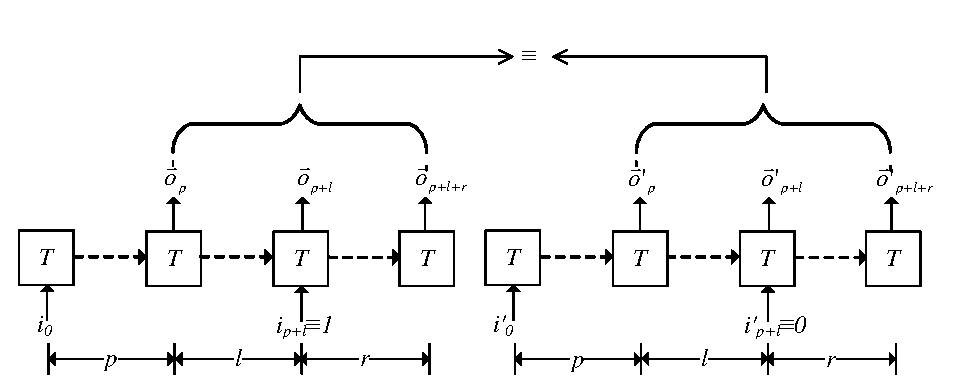
\includegraphics[width=\textwidth]{pc}
\end{center}
\caption{The under-approximative approach checking if $i_{p+l}$ can be uniquely determined}
  \label{fig_pc}
\end{figure}


Here,
$p$ is the length of the prefix state transition sequence.
$l$ and $r$ are the lengths of the two output sequences 
$<\vec{o}_{p+1},\dots,\vec{o}_{p+l}>$ and $<\vec{o}_{p+l+1},\dots,\vec{o}_{p+l+r}>$
used to determine $i_{p+l}$.
Line 1 of Equation (\ref{uniqt1}) corresponds to the left path in Figure \ref{fig_pc},
while Line 2 corresponds to the right path in Figure \ref{fig_pc}.
These two paths are of the same length.
Line 3 forces these two paths' output sequences to be the same,
while Line 4 forces their $i_{p+l}$ to be different.
\textbf{Line 5 and 6 are the assertion predicates given 
by the user that constrain the valid valuation on $\vec{i}$.
PC in $F_{PC}$ is the abbreviation of "parameterized complementary",
which means $F_{PC}(p,l,r)$ is used to check whether the encoder's input can be uniquely determined with the three parameters $p$,$l$ and $r$.
}

\textbf{
According to Figure \ref{fig_pc},
the first three lines of Equation (\ref{uniqt1}) are two unrolled transition function sequences with the same output sequences.
They can always be satisfiable with the same input variable vectors and initial state vector.
And the last two lines are constraints on input variable vectors.
We always check their satisfiability before running our algorithm.
So the unsatisfiability of $F_{PC}(p,l,r)$ always means $i_{p+l}\equiv i'_{p+l}$.
}

\textbf{According to Figure \ref{fig_pc},
it is obvious that,
if $F_{PC}(p,l,r)$ is unsatisfiable,
then $F_{PC}(p',l',r')$ is also unsatisfiable for $p'\ge p$, $l'\ge l$ and $r'\ge r$.
By studying Equation (\ref{uniqt1}),
we can find that the clause set of $F_{PC}(p',l',r')$ is a super set of $F_{PC}(p,l,r)$.
This also lead to the same conclusion.
}

\textbf{This means,
the bounded proof of $F_{PC}(p,l,r)$'s unsatisfiability
can be generalized to larger $p$, $l$ and $r$.}

\begin{proposition}\label{prop_pc1}
If $F_{PC}(p,l,r)$ is unsatisfiable,
% then $i_{p+l}$ cannot take on two different values for any particular valuation of the output sequence $<\vec{o}_{p},\dots,\vec{o}_{p+l+r}>$,
then $i_{p+l}$ can be uniquely determined by $<\vec{o}_{p},\dots,\vec{o}_{p+l+r}>$ for all larger $p$, $l$ and $r$.
\end{proposition}

\textbf{Equation (\ref{uniqt1}) does not include an initial state,
instead it use the $p$ steps prefix state transition sequence $<\vec{s_0},\dots,\vec{s_{p-1}}>$ 
to propagate the constraints $assertion(\vec{i})$ into the state sequence $<\vec{s_p},\dots,\vec{s_{p+l+r}}>$,
such that some states that can not be reached with $assertion(\vec{i})$ can be eliminated.
This leads to two major advantages over considering initial states:
First,
it simplify and speedup our algorithm by avoiding the need to compute the reachable state set or inductive invariants.
A breakthrough algorithm was proposed in \cite{TuDAC13}
to rule out unreachable states
by inferring inductive invariants.
But this algorithm can not handle our most complex XFI benchmark \cite{ShenTCAD11},
while our algorithms always can.
Second and more important,
ignoring initial states improve the decoder's reliability by 
making the decoder's output depend on only bounded history of its input.
Thus any corrupted $\vec{o}$ fed to the decoder can only affect the decoder for finite number of steps.}

\textbf{Of course ignoring initial states has one drawback that it is a little bit too stronger than necessary.
That is,
it requires that $\vec{i}$ must be uniquely determined on a larger state set $R^p$ 
that is reachable in $p$ steps from any states,
instead of on the smaller state set $R$ that is reachable from initial states.
In some cases,
our algorithm may fail to handle properly designed encoders.
% It is obvious that $R\subset R^p$.
But this has not happen on all our benchmarks from industrial applications.
% 
% Their work is orthogonal to ours.
% So to simplify our discussion,
% we will not integrate their work here.
% At the same time,
% for all the benchmarks we have tried,
% our current approach is sufficient.
}


% $d$ is the relative delay between $o_{n+d-l}^{n+d-1}$ and $i_n$,
% while $l$ is the length of $o_{n+d-l}^{n+d-1}$,
% and $p$ is the length of the prefix path used to rule out some unreachable states.
% This condition is formally defined below:

% \begin{definition11}\label{def_pcc}%\addtolength{\itemsep}{-0.5\baselineskip}
% %{\setlength{\baselineskip}{0.5\baselineskip}
% \textbf{Parameterized Complementary Condition (PC)}:
% For encoder $E$,
% assertion $R$,
% and three integers $p$,$d$ and $l$,
% $E\vDash PC(p,d,l,R)$ holds if
% \begin{enumerate}
%  \item $i_n$ can be uniquely determined by $o_{n+d-l}^{n+d-1}$ on $s_{n-p}^{n+d-1}$.
%  \item $R$ covers all $c_x$, where $n-p\le x\le n+d-1$.
% \end{enumerate}
% 
% This equals the unsatisfiability of $F_{PC}(p,d,l,R)$ in Equation (\ref{uniqt1}).
% We further define $E\vDash PC(R)$ as $\exists p,d,l:E\vDash PC(p,d,l,R)$.
% \end{definition11}

%This definition is the same as that of Subsection \ref{subsec_chkextdec} and paper \cite{ShengYuShen:iccad09}.


% At the same time,
% the last three lines of Equation (\ref{uniqt1}) correspond to Condition 2 of Definition \ref{def_pcc}.
% The 6th and the 7th lines constrain that all configuration letters are equal to $c$,
% while the last line constrains $c$ to be covered by $R$.

% The algorithm based on checking $E\vDash PC(R)$\cite{ShengYuShen:iccad09,ShengYuShen:tcad} just enumerates all combinations of $p$,$d$ and $l$,
% from small to large,
% until $F_{PC}(p,d,l,R)$ becomes unsatisfiable,
% which means that the decoder $E^{-1}$ exists.
% 
% \begin{figure}[b]
% \begin{center}
% 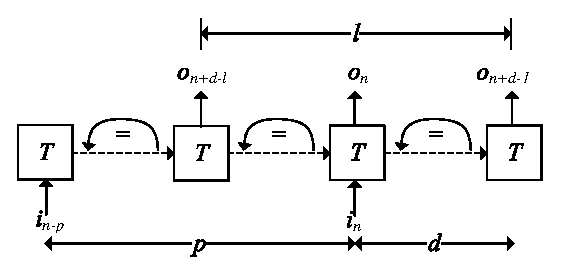
\includegraphics[width=0.45\textwidth]{doubleloop}
% \end{center}
% \caption{The loop-like non-complementary condition}
%   \label{fig_double_loop}
% \end{figure}

\subsubsection{\textbf{The over-approximative approach}}\label{subsub_complete}.

In the last subsection,
we have just learned that,
if $F_{PC}(p,l,r)$ is unsatisfiable,
then $i_{p+l}$ can be uniquely determined for all larger $p$, $l$ and $r$.
\textbf{On the other hand},
if $F_{PC}(p,l,r)$ is satisfiable,
then $i_{p+l}$ cannot be uniquely determined by $<\vec{o}_{p},\dots,\vec{o}_{p+l+r}>$ 
for this particular valuation of $p$, $l$ and $r$.
There are two possible cases:
\begin{enumerate}
 \item 
$i_{p+l}$ can be uniquely determined by $<\vec{o}_{p},\dots,\vec{o}_{p+l+r}>$ for larger $p$, $l$ and $r$;
 \item 
$i_{p+l}$ can not be uniquely determined by $<\vec{o}_{p},\dots,\vec{o}_{p+l+r}>$ for any $p$, $l$ and $r$ at all.
\end{enumerate}

If it is the first case,
then by iteratively increasing  $p$, $l$ and $r$,
$F_{PC}(p,l,r)$ will eventually become unsatisfiable.
But if it is the second case,
then this iterative algorithm will never terminate.

\begin{figure}[b]
\begin{center}
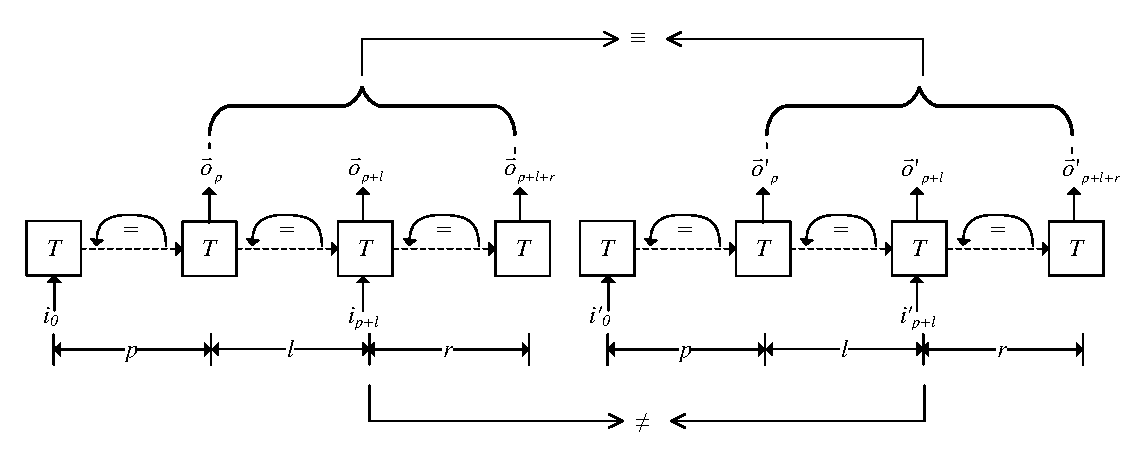
\includegraphics[width=\textwidth]{ln}
\end{center}
\caption{The over-approximative  approach checking if $i_{p+l}$ can NOT be uniquely determined}
  \label{fig_ln}
\end{figure}

So,
to obtain a halting algorithm,
we need to distinguish these two cases.
One such solution is shown in Figure \ref{fig_ln},
which is similar to Figure \ref{fig_pc} but with three additional constraints used to detect loops 
on the three state sequences $<\vec{s}_{0},\dots,\vec{s}_{p}>$,$<\vec{s}_{p+1},\dots,\vec{s}_{p+l}>$ and 
$<\vec{s}_{p+l+1},\dots,\vec{s}_{p+l+r}>$.
It is formally defined in Equation (\ref{uniqln}) with the last three lines corresponding to the three new constraints used to detect loops.

\begin{equation}\label{uniqln}
% \begin{split}
F_{LN}(p,l,r):=\\
\left\{
\begin{array}{cc}
&F_{PC}(p,l,r)\\
\wedge&\bigvee_{x=0}^{p-1}\bigvee_{y=x+1}^{p} \{\vec{s}_x\equiv \vec{s}_y\wedge \vec{s'}_x\equiv \vec{s'}_y\} \\
\wedge&\bigvee_{x=p+1}^{p+l-1}\bigvee_{y=x+1}^{p+l} \{\vec{s}_x\equiv \vec{s}_y\wedge \vec{s'}_x\equiv \vec{s'}_y\} \\
\wedge&\bigvee_{x=p+l+1}^{p+l+r-1}\bigvee_{y=x+1}^{p+l+r} \{\vec{s}_x\equiv \vec{s}_y\wedge \vec{s'}_x\equiv \vec{s'}_y\}
\end{array}
\right\}
% \end{split}
\end{equation}

\textbf{LN in $F_{LN}$ stands for "loop non-complementary",
which means $F_{LN}(p,l,r)$ with three loops is used to check whether 
the input variables can NOT be uniquely determined.
}

When $F_{LN}(p,l,r)$ is satisfiable,
then $i_{p+l}$ can \textbf{NOT} be uniquely determined by $<\vec{o}_{p},\dots,\vec{o}_{p+l+r}>$.
\textbf{More importantly,
by unrolling these three loops,
we can generalize the satisfiability of $F_{LN}(p,l,r)$ to all larger $p$, $l$ and $r$.
This means:
}

\begin{proposition}\label{prop_ln1}
If $F_{LN}(p,l,r)$ is satisfiable,
then $i_{p+l}$ cannot be uniquely determined by $<\vec{o}_{p},\dots,\vec{o}_{p+l+r}>$ for all larger $p$, $l$ and $r$.
\end{proposition}

\subsubsection{\textbf{The full algorithm}}\label{subsub_algo}.

\begin{algorithm}[b]
\SetAlgoVlined
\KwIn{The input variable $i\in\vec{i}$.}
\KwOut{whether $i\in\vec{i}$ can be uniquely determined by $\vec{o}$, and the value of $p$, $l$ and $r$.}
$p$:= 0; ~$l$:= 0;~$r$:= 0\;
\While{$1$}{
   $p$++;~$l$++;~$r$++\;\ShowLnLabel{linepc1}
   \uIf{$F_{PC}(p,l,r)$ is unsatisfiable}{
    \KwRet ($1$,$p$,$l$,$r$);\ShowLnLabel{lineln1}
   }\ShowLnLabel{lnsat}\uElseIf{$F_{LN}(p,l,r)$ is satisfiable} {
    \KwRet ($0$,$p$,$l$,$r$);
   }
}
\caption{$CheckUniqueness(i)$:The halting algorithm to determine 
whether $i\in\vec{i}$ can be uniquely determined by a bounded sequence of output variable vector $\vec{o}$}
\label{alg_pcln}
\end{algorithm}


With Propositions \ref{prop_pc1} and \ref{prop_ln1},
we can generalize their bounded proof to unbounded cases.
Thus,
we can build the halting
Algorithm \ref{alg_pcln} that determines if there exists $p$, $l$ and $r$ that enable
an input variable $i_{p+l}$ to be uniquely determined by the encoder's output sequence $<\vec{o}_{p},\dots,\vec{o}_{p+l+r}>$:
\begin{enumerate}
 \item 
On the one hand, 
if there actually exists such $p$, $l$ and $r$,
then let $p':=max(p,l,r)$,$l':=max(p,l,r)$ and $r':=max(p,l,r)$.
From Propositions \ref{prop_pc1},
we know that $F_{PC}(p',l',r')$ is unsatisfiable.
So eventually $F_{PC}(p,l,r)$ will become unsatisfiable in Line \ref{linepc1};
 \item
On the other hand,
if there does not exist such $p$, $l$ and $r$,
then eventually $p$, $l$ and $r$ will be larger than the encoder's longest path without loop,
which means that there will be three loops in $<\vec{s}_{0},\dots,\vec{s}_{p}>$,$<\vec{s}_{p+1},\dots,\vec{s}_{p+l}>$ and 
$<\vec{s}_{p+l+1},\dots,\vec{s}_{p+l+r}>$.
This will make $F_{LN}(p,l,r)$ satisfiable in Line \ref{lnsat}.
\end{enumerate}


Both cases will lead to this Algorithm's termination.

%\subsection{Removing Redundant Output Letters}\label{sec_rmred}

\section{Identifying flow control variables}\label{sec_findfc}
We will first introduce how to find out the set of flow control variables in Subsection \ref{basic},
and then introduce how to speed up this algorithm with incremental SAT in Subsection \ref{incSAT}.

\subsection{Finding out flow control variables}\label{basic}
%TODO here
To facilitate the presentation of our algorithm,
we assume that the input variable vector $\vec{i}$ can be partitioned into two vectors: 
the flow control vector $\vec{f}$ and the data vector $\vec{d}$.
And the algorithm to find out this partition will be presented in this Subsection.

% In this section,
% we propose a two-step algorithm to 
% first find out $\vec{f}$,
% and then characterize a formula over the $\vec{f}$ that makes $\vec{d}$ to be uniquely determined by the encoder's output variable vector $\vec{o}$.
% 
% \subsection{}

The flow control vector $\vec{f}$ are used to represent the validness of $\vec{d}$.
So,
for a properly designed encoder,
$\vec{f}$ should always be uniquely determined by a bounded sequence of the encoder's output variable vector $\vec{o}$,
or else the decoder cannot recognize the validness of $\vec{d}$.

\begin{algorithm}[b]
\SetAlgoVlined
\KwIn{The input variable vector $\vec{i}$.}
\KwOut{$\vec{f}\subset \vec{i}$ and $\vec{d}\subset \vec{i}$  that can and can not 
be uniquely determined ,and the maximal $p$, $l$ and $r$ .}
\ShowLnLabel{initfd}$\vec{f}: = \{\}$;$\vec{d}:= \{\}$\;
\ShowLnLabel{initplr}$p$:= 0 ;~$l$:= 0 ;~$r$:= 0 \;
\ShowLnLabel{while}\While{$\vec{i}\ne \{\}$}{
  $p++$; ~ $l++$; ~ $r++$\;
  assume $i\in\vec{i}$\;
  \uIf {$F_{PC}(p,l,r)$ is unsatisfiable for $i$} {
    \ShowLnLabel{adduniq}
    $\vec{f}:= i\cup\vec{f}$\;
    $\vec{i}:=\vec{i}-i$\;
  }\ShowLnLabel{nonuniqres}
  \uElseIf {$F_{LN}(p,l,r)$ is satisfiable for  $i$ and assume its satisfying assignment is $A$}{
    \ForEach{$j\in\vec{i}$} {
\ShowLnLabel{ruleout}      \If {$A(j_{p+l})\neq A(j'_{p+l})$} {
	$\vec{i}:=\vec{i}-j$\;
	$\vec{d}:=j\cup\vec{d}$
      }
    }
  }
}
\KwRet ($\vec{f}$,$p_{max}$,$l_{max}$,$r_{max}$)
\caption{$FindFlow(\vec{i})$:Identifying the flow control vector}
\label{alg_fofc}
\end{algorithm}

Thus,
Algorithm \ref{alg_fofc} is proposed to identify $\vec{f}$.

At Line \ref{initfd},
the initial value of $f$ and $d$ are set to empty vector.
At Line \ref{initplr},
the initial value of $p$, $l$ and $r$ are all set to 0.

At Line \ref{while},
a while loop is used to iterate on all $i\in\vec{i}$.

At Line \ref{adduniq},
the input variable $i$ that can be uniquely determined will be added to the vector $\vec{f}$.

On the other hand,
when $\vec{i}$ is very long,
the run time overhead of testing each $i\in\vec{i}$ one by one would also be very large.
To speed up this testing procedure,
when $F_{LN}(p,l,r)$ is satisfiable at Line \ref{nonuniqres},
every $j\in\vec{i}$ that has different values for $j_{p+l}$ and $j'_{p+l}$ 
in the satisfying assignment of $F_{LN}(p,l,r)$ can also be moved to $\vec{d}$ at Line \ref{ruleout},
because their own $F_{LN}(p,l,r)$ is also satisfiable.

\textbf{In some particular case,
some data variable $d\in \vec{d}$ can be uniquely determined,
just like a flow control variable $f\in \vec{f}$.
In this case,
$d$ may be identified as a flow control variable by Algorithm \ref{alg_fofc}.
But this do not harm our overall framework,
because the decoder's Boolean function can still be correctly characterized in Section \ref{sec_char}.
}


\subsection{Speeding up with incremental SAT}\label{incSAT}

We can further speedup Algorithm \ref{alg_fofc} by employing the MiniSat's incremental SAT mechanism mentioned in Subsection \ref{subsec_incsat}.

$F_{PC}(p,l,r)$ in Equation \ref{uniqt1} can be partitioned into the following two equations:
\begin{equation}\label{uniqt1_f}
% \begin{split}
C_{PC}(p,l,r):=
\left\{
\begin{array}{cc}
&\bigwedge_{m=0}^{p+l+r}
\{
(\vec{s}_{m+1},\vec{o}_m)\equiv T(\vec{s}_m,\vec{i}_m)
\}
\\
\wedge&\bigwedge_{m=0}^{p+l+r}
\{
(\vec{s'}_{m+1},\vec{o'}_m)\equiv T(\vec{s'}_m,\vec{i'}_m)
\}
\\
\wedge&\bigwedge_{m=p}^{p+l+r}\vec{o}_m\equiv \vec{o'}_m \\
\wedge&\bigwedge_{m=0}^{p+l+r}assertion(\vec{i}_m) \\
\wedge&\bigwedge_{m=0}^{p+l+r}assertion(\vec{i'}_m) 
\end{array}
\right\}
% \end{split}
\end{equation}

\begin{equation}\label{uniqt1_a}
% \begin{split}
A_{PC}(p,l,r):=
\left\{
\begin{array}{c}
 i_{p+l}\equiv 1 \wedge  i'_{p+l}\equiv 0 
\end{array}
\right\}
% \end{split}
\end{equation}

\begin{algorithm}[b]
\SetAlgoVlined
\KwIn{The input variable vector $\vec{i}$.}
\KwOut{$\vec{f}\subset \vec{i}$ and $\vec{d}\subset \vec{i}$ that can and can not 
be uniquely determined,
and the maximal $p$, $l$ and $r$ .}
\ShowLnLabel{initfd2}$\vec{f}: = \{\}$;$\vec{d}:= \{\}$\;
\ShowLnLabel{initplr2}$p$:= 0 ;~$l$:= 0 ;~$r$:= 0 \;
\ShowLnLabel{while2}\While{$\vec{i}\ne \{\}$}{
  $p++$; ~ $l++$; ~ $r++$\;
\ShowLnLabel{addcls21}  $addClause(C_{PC}(p,l,r))$\;
  \ForEach{$i\in\vec{i}$} {
\ShowLnLabel{solve21}    \If {$solve(A_{PC}(p,l,r))$ is unsatisfiable for $i$} {
      \ShowLnLabel{adduniq2}
      $\vec{i}:= \vec{i}-i$\;
      $\vec{f}:= i\cup\vec{f}$\;
    }
  }
\ShowLnLabel{addcls22}  $addClause(C_{LN}(p,l,r))$\;
  \ForEach{$i\in\vec{i}$} {
\ShowLnLabel{solve22}    \If {$solve(A_{LN}(p,l,r))$ is satisfiable for $i$ and satisfying assignment is $A$} {
      \ShowLnLabel{adduniq3}
      \ForEach{$j\in\vec{i}$} {
\ShowLnLabel{ruleout2}      \If {$A(j_{p+l})\neq A(j'_{p+l})$} {
	  $\vec{i}:=\vec{i}-j$\;
	  $\vec{d}:=j\cup\vec{d}$
	}
      }
    }
  }
}
\KwRet ($\vec{f}$,$p$,$l$,$r$)
\caption{$FindFlowIncSAT(\vec{i})$:Identifying the flow control vector with incremental SAT}
\label{alg_fofc_inc}
\end{algorithm}

Similarly we can partition $F_{LN}(p,l,r)$ in Equation \ref{uniqln} into the following two equations:

\begin{equation}\label{uniqln_f}
% \begin{split}
C_{LN}(p,l,r):=\\
\left\{
\begin{array}{cc}
&C_{PC}(p,l,r)\\
\wedge&\bigvee_{x=0}^{p-1}\bigvee_{y=x+1}^{p} \{\vec{s}_x\equiv \vec{s}_y\wedge \vec{s'}_x\equiv \vec{s'}_y\} \\
\wedge&\bigvee_{x=p+1}^{p+l-1}\bigvee_{y=x+1}^{p+l} \{\vec{s}_x\equiv \vec{s}_y\wedge \vec{s'}_x\equiv \vec{s'}_y\} \\
\wedge&\bigvee_{x=p+l+1}^{p+l+r-1}\bigvee_{y=x+1}^{p+l+r} \{\vec{s}_x\equiv \vec{s}_y\wedge \vec{s'}_x\equiv \vec{s'}_y\}
\end{array}
\right\}
% \end{split}
\end{equation}

\begin{equation}\label{uniqln_a}
% \begin{split}
A_{LN}(p,l,r):=
\left\{
\begin{array}{c}
 i_{p+l}\equiv 1 \wedge  i'_{p+l}\equiv 0 
\end{array}
\right\}
% \end{split}
\end{equation}



It is obvious that $C_{PC}$ and $C_{LN}$ are independent of any particular $i\in \vec{i}$,
so they can be added into the clause database of MiniSat solver by calling $addClause(C_{PC})$ or $addClause(C_{LN})$.
At the same time, 
all clauses in $A_{PC}$ and $A_{LN}$ contain only one literal,
so they can be used as the assumptions in calling $solve$ procedure of MiniSat solver.

Thus,
with these new equations,
we can change Algorithm \ref{alg_fofc} to Algorithm \ref{alg_fofc_inc} with incremental SAT.
The major changes are the two new $addClause$ in Line \ref{addcls21} and \ref{addcls22},
and the two new $solve$ in Line \ref{solve21} and \ref{solve22}.
They are the procedures provided by MiniSat's incremental SAT mechanism mentioned in Subsection \ref{subsec_incsat}.





% 
% \subsection{Reducing the value of $p$ $l$ and $r$}\label{reduceing}
% 
% 
% \begin{algorithm}[b]
% \SetAlgoVlined
% \KwIn{The valuation of $p$, $l$ and $r$.}
% \KwOut{The minmal valuation of $l$ and $r$ that can still make $F_{PC}(p,l,r)$ unsatisfiable.}
% \For{$r'=r \to 1$} {
% \ShowLnLabel{checkrsat}  \If{$F_{PC}(p,l,r'-1)$ is satisfiable} {
%     break
%   }
%   \ElseIf{$r'\equiv 1$} {
%     $r':=r'-1$\\
%     break
%   }
% }
% \For{$l'=l \to 1$} {
%   \If{$F_{PC}(p,l'-1,r')$ is satisfiable} {
%     break
%   }
%   \ElseIf{$l'\equiv 1$} {
%     $l':=l'-1$\\
%     break
%   }
% }
% return $<d',l'>$
% \caption{$RemoveRedundancy(p,l,r)$}
% \label{algo_remove}
% \end{algorithm}
% 
% \textbf{
% Although Algorithm \ref{alg_fofc_inc} is sufficient to determine whether $i$ can be uniquely determined,
% there are some redundancy in the valuations of $<p,d,l>$ found by it,
% which may cause unnecessarily large overheads on the circuit area.}
% 
% 
% \textbf{
% Thus,
% we use Algorithm \ref{algo_remove} to minimize $l$ and $r$ one by one.
% For each $r'$,
% $r'-1$ is used to checked for $F_{PC}$'s satisfiability at Line \ref{checkrsat}.
% If it is satisfiable,
% $l'$ is returned because it is the smallest $l$ that can make $F_{PC}(p,l,r)$ unsatisfiable.
% On the other hand,
% if it is unsatisfiable but $l'$ already reach $1$,
% then terminate and return 0.
% $l$ is handled similarly.
% }
% 

%Please refer to \cite{ShenTCAD11} for more details.



\section{Inferring predicate that enables the encoder's data vector to be uniquely determined}\label{sec_infer}

% Furthermore,
% the validness of $\vec{d}$ is indicated by a predicate $valid(\vec{f})$.
% So for a properly designed encoder,
% $valid(\vec{f})$ should make $\vec{d}$ to be uniquely determined by the encoder's output.

In Subsection \ref{subsec_craig},
we propose  an algorithm 
to characterize a Boolean function that makes a Boolean formula satisfiable.
In Subsection \ref{subsec_infer},
we apply this algorithm to infer $valid(\vec{f})$,
the predicate that enable $\vec{d}$ to be uniquely determined by a bounded sequence of $\vec{o}$.


\subsection{Characterizing a function that makes a Boolean formula satisfiable}\label{subsec_craig}

Assume that $R(\vec{a},\vec{b},t)$ is a Boolean formula with $R(\vec{a},\vec{b},0)\wedge R(\vec{a},\vec{b},1)$ unsatisfiable.
% That is,
% $\vec{a}$ and $\vec{b}$ uniquely determine $t$.
$\vec{a}$ and $\vec{b}$ are respectively called the important and the non-important variable vectors,
while $t$ is the target variable.

We need to characterize a Boolean function $FSAT_R(\vec{a})$,
which covers and only covers all the valuations of $\vec{a}$ 
that can make $R(\vec{a},\vec{b},1)$ satisfiable.
It is formally defined below:

\begin{equation}\label{fchar}
% \begin{split}
FSAT_R(\vec{a}):=
\left\{
\begin{array}{rcl}
1 & & \exists\vec{b}.R(\vec{a},\vec{b},1) \\
0 & & otherwise
\end{array}
\right.
% \end{split}
\end{equation}
%% HAHA come to here

Thus,
a naive algorithm of computing $FSAT_R(\vec{a})$ is to enumerate all valuations of $\vec{a}$,
and collect all those valuations that make $R(\vec{a},\vec{b},1)$ satisfiable.
But the number of valuations to be enumerated is $2^{|\vec{a}|}$,
which will prevent this algorithm from terminating within reasonable time for a large $\vec{a}$.

We can speed up this naive algorithm by expanding each valuation of $\vec{a}$ to a larger set with cofactoring \cite{EFFSATUSMCCO} and Craig interpolant\cite{interp_McMillan}.
Intuitively,
assume that $R(\vec{a},\vec{b},1)$ is satisfiable with a satisfying assignment $A:\vec{a}\cup\vec{b}\cup\{t\}\to\{0,1\}$,
the following new formula can be constructed by cofactoring\cite{EFFSATUSMCCO}:

\begin{algorithm}[t]
\SetAlgoVlined
\KwIn{The Boolean formula $R(\vec{a},\vec{b},t)$, 
its important variable vector $\vec{a}$,
its non-important variable vector $\vec{b}$,
and its target variable $t$.}
\KwOut{$FSAT_R(\vec{a})$ that makes $R(\vec{a},\vec{b},1)$ satisfiable.}
\ShowLnLabel{initcondition}
$FSAT_R(\vec{a}):= 0$ \;
\ShowLnLabel{testsat}
\While { $R(\vec{a},\vec{b},1)\wedge\neg FSAT_R(\vec{a})$ is satisfiable } {
  assume $A:\vec{a}\cup\vec{b}\cup\{t\}\rightarrow \{0,1\}$ is the satisfying assignment \;
\ShowLnLabel{cofact1}
  $\phi_A(\vec{a}):= R(\vec{a},A(\vec{b}),1)$ \;
\ShowLnLabel{cofact2}
  $\phi_B(\vec{a}):= R(\vec{a},A(\vec{b}),0)$ \;
\ShowLnLabel{ab}
  assume $ITP(\vec{a})$ is the Craig interpolant of $\phi_A$ with respect to $\phi_B$ \;
\ShowLnLabel{add}
  $FSAT_R(\vec{a}):= ITP(\vec{a}) \vee FSAT_R(\vec{a})$ \;
}
\KwRet $FSAT_R(\vec{a})$
\caption{$CharacterizingFormulaSAT(R,\vec{a},\vec{b},t)$:Characterizing a Boolean function over $\vec{a}$ that can make $R(\vec{a},\vec{b},1)$ satisfiable}
\label{alg_craigchar}
\end{algorithm}

\begin{equation}
% \begin{split}
R(\vec{a},A(\vec{b}),1):=R(\vec{a},\vec{b},1)_{b\equiv A(b)}
% \end{split}
\end{equation}

Because $R(\vec{a},A(\vec{b}),0)\wedge R(\vec{a},A(\vec{b}),1)$ is unsatisfiable,
the Craig interpolant $ITP(\vec{a})$ of $R(\vec{a},A(\vec{b}),1)$ with respect to $R(\vec{a},A(\vec{b}),0)$ can be computed 
and used as an over-approximation of the set of $\vec{a}$ that makes $R(\vec{a},A(\vec{b}),1)$ satisfiable.
At the same time,
$ITP(\vec{a})\wedge R(\vec{a},A(\vec{b}),0)$ is unsatisfiable,
so $ITP(\vec{a})$ covers nothing that can make $R(\vec{a},A(\vec{b}),0)$ satisfiable.
Thus,$ITP(\vec{a})$ covers exactly the set of valuations of $\vec{a}$ that can make $R(\vec{a},A(\vec{b}),1)$ satisfiable.


Based on the foregoing discussion,
Algorithm \ref{alg_craigchar} is proposed to characterize $FSAT_R(\vec{a})$ in Equation (\ref{fchar}).
Line \ref{testsat} checks whether there is still some new valuation of $\vec{a}$ that can make $R(\vec{a},\vec{b},1)$ satisfiable,
but has not been covered by $FSAT_R(\vec{a})$.
Lines \ref{cofact1} and \ref{cofact2} assign the value of $\vec{b}$ 
from the satisfying assignment to $R(\vec{a},\vec{b},1)$ and $R(\vec{a},\vec{b},0)$ respectively, 
to remove $\vec{b}$ from them.

Thus,
$\phi_A\wedge \phi_B$ in Line \ref{ab} is unsatisfiable,
and the common variables vector of $\phi_A$ and $\phi_B$ is $\vec{a}$.
So a Craig interpolant $ITP(\vec{a})$ can be generated with the McMillian's algorithm\cite{interp_McMillan}.

$ITP(\vec{a})$ is added to $FSAT_R(\vec{a})$ in Line \ref{add} and ruled out in Line \ref{testsat} again.

Each iteration of the while loop in Algorithm \ref{alg_craigchar} adds at least a valuation of $\vec{a}$ to $FSAT_R(\vec{a})$,
which means that $FSAT_R(\vec{a})$ is a Boolean function that covers a bounded and strictly increasing set of valuations of $\vec{a}$.
So Algorithm \ref{alg_craigchar} is a halting one.

\subsection{Inferring $valid(\vec{f})$ that enables $\vec{d}$ to be uniquely determined}\label{subsec_infer}
% This subsection introduces the non-trivial details of how to infer the predicate $valid(\vec{f})$.
% So we first present an intuitive and informal introduction in \ref{subsub_intro}.
% And then present its details in \ref{subsub_nonloop}, \ref{subsub_loop} and \ref{subsub_overal}.

% \subsubsection{\textbf{Intuitive introduction}}\label{subsub_intro}.

In this Section,
we will present how to compute the predicate $valid(\vec{f})$ that enables $\vec{d}$ to be uniquely determined.
Similar to the halting algorithm presented in Subsection \ref{subsec_chkextdec},
we will first present how to compute a monotonically growing under-approximation of $valid(\vec{f})$ in \ref{subsub_nonloop},
and them present how to compute a monotonically shrinking over-approximation of $valid(\vec{f})$ in \ref{subsub_loop},
and finally show that they will converge to $valid(\vec{f})$ in \ref{subsub_overal}.


% 
% With Algorithm \ref{alg_craigchar} we can find out $FSAT_{F_{PC}}(\vec{f}_{p+l})$, 
% the set of 
% valuation of $\vec{f}_{p+l}$ that can make $F_{PC}(p,l,r)$ satisfiable for a particular $p$,$l$ and $r$.
% So its negation $\neg FSAT_{F_{PC}}(\vec{f}_{p+l})$ seems to be what we want.
% 
% As shown intuitively in Figure \ref{fig_mono},
% $\neg FSAT_{F_{PC}}(\vec{f}_{p+l})$ is an under-approximation of $valid(\vec{f})$
% that grow monotonically with respect to $p$,$l$ and $r$.
% We will prove this in \ref{subsub_nonloop}.
% So we still need an over-approximation of $valid(\vec{f})$ 
% that shrinks monotonically with respect to $p$,$l$ and $r$ to construct a halting algorithm,
% which will be presented in \ref{subsub_loop}.



% % We call the predicate that cover and only cover this set $FSAT_{PC}(p,l,r)$.
% % And we will present how to infer it in \ref{subsub_nonloop}.
% 
% % But as shown in Subsection \ref{subsec_chkextdec},
% % from the fact that $\vec{d}$ is uniquely determined for some particular $p$,$l$ and $r$,
% % we can only know that it is also uniquely determined for all larger $p'$,$l'$ and $r'$.
% % On the other hand,
% But according to Figure \ref{fig_pc} and Proposition \ref{prop_pc1},
% only the unsatisfiability of $F_{PC}(p,l,r)$ can be generalized to larger $p$,$l$ and $r$,
% while its satisfiability can not.
% % $\vec{d}_{p+l}$ not uniquely determined for some particular $p$,$l$ and $r$,
% % may become uniquely determined for larger $p$,$l$ and $r$.
% % For example,
% % an encoder with 3 step latency can not uniquely determine its input $\vec{i}$ with $p$,$l$ and $r$ smaller than 3.
% % But it can with $p$,$l$ and $r$ larger than 3.
% % That means,
% This means,
% a particular valuation of $\vec{f}_{p+l}$ that 
% makes $F_{PC}(p,l,r)$ satisfiable for some $p$,$l$ and $r$,
% may make it unsatisfiable for some larger $p$,$l$ and $r$.
% 
% So as shown in Figure \ref{fig_mono}, 
% $FSAT_{F_{PC}}(\vec{f}_{p+l})$ is a set monotonically shrinking with respect to $p$,$l$ and $r$,
% which make its negation $\neg FSAT_{PC}(p,l,r)$ an under-approximation of $valid(\vec{f})$
% that grow monotonically with respect to $p$,$l$ and $r$.
% We still need an over-approximation that shrink monotonically to construct a halting algorithm.


% Inspired by the Figure \ref{fig_ln} and $F_{LN}(p,l,r)$,
% we can compute this over-approximation by using Algorithm \ref{alg_craigchar} 
% to find out the set of valuation of $\vec{f}_{p+l}$ that can make $F_{LN}(p,l,r)$ satisfiable.
% We call the predicate that covers and only covers this set $FSAT_{LN}(p,l,r)$.
% With a satisfiable $F_{LN}(p,l,r)$,
% by unrolling the three loops in Figure \ref{fig_ln},
% we can prove that $F_{LN}(p,l,r)$ is still satisfiable for larger $p$,$l$ and $r$.
% That means $FSAT_{LN}(p,l,r)$ is a set of valuation of $\vec{f}_{p+l}$ that makes $F_{LN}(p,l,r)$ satisfiable 
% and grows monotonically with respect to $p$,$l$ and $r$.
% So as shown in Figure \ref{fig_mono},
% $\neg FSAT_{LN}(p,l,r)$ is an over-approximation of $valid(\vec{f})$ that shrinks monotonically.
% We will present how to infer it in \ref{subsub_loop}.
% 
% Together with these two inferred predicates,
% an iterative algorithm is presented in \ref{subsub_overal} to infer $valid(\vec{f})$.

\subsubsection{\textbf{Computing monotonically growing under-approximation of $valid(\vec{f})$}}\label{subsub_nonloop}.

By replacing $i$ in Equation (\ref{uniqt1}) with $\vec{d}$,
we have:

\begin{equation}\label{uniqt1d}
% \begin{split}
F^d_{PC}(p,l,r):=
\left\{
\begin{array}{cc}
&\bigwedge_{m=0}^{p+l+r}
\{
(\vec{s}_{m+1},\vec{o}_m)\equiv T(\vec{s}_m,\vec{i}_m)
\}
\\
\wedge&\bigwedge_{m=0}^{p+l+r}
\{
(\vec{s'}_{m+1},\vec{o'}_m)\equiv T(\vec{s'}_m,\vec{i'}_m)
\}
\\
\wedge&\bigwedge_{m=p}^{p+l+r}\vec{o}_m\equiv \vec{o'}_m \\
\wedge& \vec{d}_{p+l}\ne \vec{d}'_{p+l} \\
\wedge&\bigwedge_{m=0}^{p+l+r}assertion(\vec{i}_m) \\
\wedge&\bigwedge_{m=0}^{p+l+r}assertion(\vec{i'}_m) 
\end{array}
\right\}
% \end{split}
\end{equation}

If $F^d_{PC}(p,l,r)$ is satisfiable,
then $\vec{d}_{p+l}$ cannot be uniquely determined by $<\vec{o}_p,\dots,\vec{o}_{p+l+r}>$.
We define a new formula $T_{PC}(p,l,r)$ by collecting the 3rd line of Equation (\ref{uniqt1d}):

\begin{equation}\label{tpc}
% \begin{split}
T_{PC}(p,l,r):=\\
\left\{
\begin{array}{cc}
      &\bigwedge_{m=p}^{p+l+r}\vec{o}_m\equiv \vec{o'}_m \\
\end{array}
\right\}
% \end{split}
\end{equation}

By substituting $T_{PC}(p,l,r)$ back into $F^d_{PC}(p,l,r)$,
we have a new formula:
\begin{equation}\label{fpcq}
% \begin{split}
F'^d_{PC}(p,l,r,t):=
\left\{
\begin{array}{cc}
&\bigwedge_{m=0}^{p+l+r}
\{
(\vec{s}_{m+1},\vec{o}_m)\equiv T(\vec{s}_m,\vec{i}_m)
\}
\\
\wedge&\bigwedge_{m=0}^{p+l+r}
\{
(\vec{s'}_{m+1},\vec{o'}_m)\equiv T(\vec{s'}_m,\vec{i'}_m)
\}
\\
\wedge& t\equiv T_{PC}(p,l,r)\\
\wedge& \vec{d}_{p+l}\ne \vec{d'}_{p+l} \\
\wedge&\bigwedge_{m=0}^{p+l+r}assertion(\vec{i}_m) \\
\wedge&\bigwedge_{m=0}^{p+l+r}assertion(\vec{i'}_m) 
\end{array}
\right\}
% \end{split}
\end{equation}


Obviously $F^d_{PC}(p,l,r)$ and $F'^d_{PC}(p,l,r,1)$ are equivalent.
% $\vec{d}$ cannot be uniquely determined for a particular valuation of $p$, $l$ and $r$ if $F'_{PC}(p,l,r,1)$ is satisfiable.
We further define:

% By comparing Equation (\ref{fpcq}),
% it is obvious that $F_{PC}(p,l,r)$ in Equation (\ref{uniqt1}) can be reformulated as: 
% \begin{equation}\label{fpcref}
% % \begin{split}
% F_{PC}(p,l,r):=F'_{PC}(p,l,r,t)\wedge (t\equiv 1)
% \end{equation}
% 
% $\vec{f}_{p+l}$ can be uniquely determined by $<\vec{o}_p,\dots,\vec{o}_{p+l+r}>$,
% so $\vec{f}_{p+l}\equiv \vec{f'}_{p+l}$ always holds.
% Thus,
% $\vec{i}_{p+l}\ne \vec{i'}_{p+l}$ in Line 3 of Equation (\ref{fpcq}) should be reformulated as $\vec{d}_{p+l}\ne \vec{d'}_{p+l}$.


% Thus,
% to use Algorithm \ref{alg_craigchar} to characterize the formula over $\vec{f}_{p+l}$ that makes $F'_{PC}(p,l,r,1)$ satisfiable,
% we can define the following equation:
\begin{equation}\label{pcdef1}
\vec{a}:=\vec{f}_{p+l}
\end{equation}

\begin{equation}\label{pcdef2}
\vec{b}:=\vec{d}_{p+l}\cup \vec{d'}_{p+l}\cup \vec{s}_0\cup \vec{s'}_0\cup\bigcup_{0\le x\le p+l+r,x\neq (p+l)}(\vec{i}_{x}\cup\vec{i'}_{x})
\end{equation}

% $\vec{f}_{p+l}$ can be uniquely determined, 
% so we do not need to consider $\vec{f'}_{p+l}$.
Thus,
$\vec{a}\cup\vec{b}$ is the vector that contains all the input variable vectors $<\vec{i}_0,\dots,\vec{i}_{p+l+r}>$ and $<\vec{i'}_0,\dots,\vec{i'}_{p+l+r}>$
at all steps for the two sequences of unrolled transition function.
It also contains the two initial states $\vec{s}_0$ and $\vec{s'}_0$.
In addition,
the transition function $T$ in the first two lines of Equation (\ref{fpcq})
is a function that computes the next state and the output variable vector from the current state and input variable vector.
So $\vec{a}$ and $\vec{b}$ can uniquely determine the value of $t$ in $F'^d_{PC}(p,l,r,t)$.
Thus,
for a particular combination of $p$,$l$ and $r$,
the Boolean function over $\vec{f}_{p+l}$ that makes $F'^d_{PC}(p,l,r,1)$ satisfiable can be computed 
by calling Algorithm \ref{alg_craigchar} with $F'^d_{PC}(p,l,r,t)$, $\vec{a}$ and $\vec{b}$ defined above:

\begin{equation}\label{fsat_pc}
FSAT_{PC}(p,l,r):=CharacterizingFormulaSAT(F'^d_{PC}(p,l,r,t),\vec{a},\vec{b},t)
\end{equation}

So $FSAT_{PC}(p,l,r)$ is the set of $\vec{f}_{p+l}$ 
that makes $F^d_{PC}(p,l,r)$ satisfiable.
Thus,
its negation $\neg FSAT_{PC}(p,l,r)$ is the set of $\vec{f}_{p+l}$ 
that makes $F^d_{PC}(p,l,r)$ unsatisfiable.

Again according to Proposition \ref{prop_pc1},
the unsatisfiable proof of $F^d_{PC}(p,l,r)$ can be generalized to all larger $p$,$l$ and $r$.
So every valuation of $\vec{f}$ covered by $\neg FSAT_{PC}(p,l,r)$ can also make $F^d_{PC}(p,l,r)$ unsatisfiable for all larger $p$,$l$ and $r$.

So we have:

\begin{proposition}\label{prop_pc}
$\neg FSAT_{PC}(p,l,r)$ is an under-approximation of $valid(\vec{f})$ that grow monotonically with respect to $p$,$l$ and $r$.
\end{proposition}


\begin{figure}[t]
\begin{center}

\includegraphics[width=0.5\textwidth]{mono}
\end{center}
\caption{The monotonicity of $FSAT_{PC}(p,l,r)$ and $FSAT_{LN}(p,l,r)$}
  \label{fig_mono}
\end{figure}



This is shown intuitively in Figure \ref{fig_mono}..

\subsubsection{\textbf{Computing monotonically shrinking over-approximation of $valid(\vec{f})$}}\label{subsub_loop}.

Similarly,
by replacing $i$ in $F_{LN}(p,l,r)$ of Equation (\ref{uniqln}) with $\vec{d}$,
we have:

\begin{equation}\label{uniqlnd}
% \begin{split}
F^d_{LN}(p,l,r):=\\
\left\{
\begin{array}{cc}
&\bigwedge_{m=0}^{p+l+r}
\{
(\vec{s}_{m+1},\vec{o}_m)\equiv T(\vec{s}_m,\vec{i}_m)
\}
\\
\wedge&\bigwedge_{m=0}^{p+l+r}
\{
(\vec{s'}_{m+1},\vec{o'}_m)\equiv T(\vec{s'}_m,\vec{i'}_m)
\}
\\
\wedge&\bigwedge_{m=p}^{p+l+r}\vec{o}_m\equiv \vec{o'}_m \\
\wedge& \vec{d}_{p+l}\ne \vec{d}'_{p+l} \\
\wedge&\bigwedge_{m=0}^{p+l+r}assertion(\vec{i}_m) \\
\wedge&\bigwedge_{m=0}^{p+l+r}assertion(\vec{i'}_m) \\
\wedge&\bigvee_{x=0}^{p-1}\bigvee_{y=x+1}^{p} \{\vec{s}_x\equiv \vec{s}_y\wedge \vec{s'}_x\equiv \vec{s'}_y\} \\
\wedge&\bigvee_{x=p+1}^{p+l-1}\bigvee_{y=x+1}^{p+l} \{\vec{s}_x\equiv \vec{s}_y\wedge \vec{s'}_x\equiv \vec{s'}_y\} \\
\wedge&\bigvee_{x=p+l+1}^{p+l+r-1}\bigvee_{y=x+1}^{p+l+r} \{\vec{s}_x\equiv \vec{s}_y\wedge \vec{s'}_x\equiv \vec{s'}_y\}
\end{array}
\right\}
% \end{split}
\end{equation}

If $F^d_{LN}(p,l,r)$ is satisfiable,
then $\vec{d}_{p+l}$ cannot be uniquely determined by $<\vec{o}_p,\dots,\vec{o}_{p+l+r}>$.
Furthermore,
similar to Proposition \ref{prop_ln1},
by unrolling those three loops in the last three lines of Equation (\ref{uniqlnd}),
we can prove that $\vec{d}_{p+l}$ cannot be uniquely determined for any larger $p$,$l$ and $r$.
We further define a new formula $T_{LN}(p,l,r)$ by collecting the 3rd line and the last three lines of Equation (\ref{uniqlnd}):

\begin{equation}\label{tln}
% \begin{split}
T_{LN}(p,l,r):=\\
\left\{
\begin{array}{cc}
      &\bigwedge_{m=p}^{p+l+r}\vec{o}_m\equiv \vec{o'}_m \\
\wedge&\bigvee_{x=0}^{p-1}\bigvee_{y=x+1}^{p} \{\vec{s}_x\equiv \vec{s}_y\wedge \vec{s'}_x\equiv \vec{s'}_y\} \\
\wedge&\bigvee_{x=p+1}^{p+l-1}\bigvee_{y=x+1}^{p+l} \{\vec{s}_x\equiv \vec{s}_y\wedge \vec{s'}_x\equiv \vec{s'}_y\} \\
\wedge&\bigvee_{x=p+l+1}^{p+l+r-1}\bigvee_{y=x+1}^{p+l+r} \{\vec{s}_x\equiv \vec{s}_y\wedge \vec{s'}_x\equiv \vec{s'}_y\}
\end{array}
\right\}
% \end{split}
\end{equation}

By replacing the 3rd line and the last three lines of Equation (\ref{uniqlnd}) with $T_{LN}(p,l,r)$,
we got:

\begin{equation}\label{lndef1}
F'^d_{LN}(p,l,r,t):=
\left\{
\begin{array}{cc}
&\bigwedge_{m=0}^{p+l+r}
\{
(\vec{s}_{m+1},\vec{o}_m)\equiv T(\vec{s}_m,\vec{i}_m)
\}
\\
\wedge&\bigwedge_{m=0}^{p+l+r}
\{
(\vec{s'}_{m+1},\vec{o'}_m)\equiv T(\vec{s'}_m,\vec{i'}_m)
\}
\\
% \wedge& \vec{f}_{p+l}\equiv \vec{f'}_{p+l}\\
\wedge& t\equiv T_{LN}(p,l,r)\\
\wedge& \vec{d}_{p+l}\ne \vec{d'}_{p+l} \\
\wedge&\bigwedge_{m=0}^{p+l+r}assertion(\vec{i}_m) \\
\wedge&\bigwedge_{m=0}^{p+l+r}assertion(\vec{i'}_m) 
\end{array}
\right\}
\end{equation}

Obviously $F^d_{LN}(p,l,r)$ and $F'^d_{LN}(p,l,r,1)$ are equivalent.
Thus,
for a particular valuation of $p$,$l$ and $r$,
the function over $\vec{f}_{p+l}$ that makes $F^d_{LN}(p,l,r)$ satisfiable can be 
computed by 

\begin{equation}\label{fsat_ln}
FSAT_{LN}(p,l,r):=CharacterizingFormulaSAT(F'^d_{LN}(p,l,r,t),\vec{a},\vec{b},t)
\end{equation}

Again according to Proposition \ref{prop_ln1},
the satisfiable proof of $F^d_{LN}(p,l,r)$ can be generalized to all larger $p$,$l$ and $r$.
So every valuation of $\vec{f}$ covered by $FSAT_{LN}(p,l,r)$ can also make $F^d_{LN}(p,l,r)$ satisfiable for all larger $p$,$l$ and $r$.
So $FSAT_{LN}(p,l,r)$ grow monotonically,
and is a subset of $\neg valid(\vec{f})$.

Thus we have the following proposition:

\begin{proposition}\label{prop_ln}
$\neg FSAT_{LN}(p,l,r)$ is an over-approximation of $valid(\vec(f))$ that shrinks monotonically.
\end{proposition}

This is shown intuitively in Figure \ref{fig_mono}.

% It is obvious that $FSAT_{LN}(p,l,r)\to FSAT_{PC}(p,l,r)$.
% Thus,
% for a particular valuation of $p$, $l$ and $r$,
% if $\neg FSAT_{LN}(p,l,r)\wedge FSAT_{PC}(p,l,r)$ is unsatisfiable,
% then $\neg FSAT_{LN}(p,l,r)$ is the formula over $\vec{f}_{p+l}$ that makes $\vec{d}_{p+l}$ to be uniquely determined by the encoder's output sequence.


\subsubsection{\textbf{The algorithm to compute $valid(\vec{f})$}}\label{subsub_overal}.

\begin{algorithm}[t]
\SetAlgoNoLine
% \KwIn{The Boolean formula $R(\vec{a},\vec{b},t)$, 
% its important variable vector $\vec{a}$,
% its non-important variable vector $\vec{b}$,
% and its target variable $t$.}
% \KwOut{$F_i(\vec{a})$ that makes $R(\vec{a},\vec{b},1)$ satisfiable.}
$p$:= $p_{max}$;~$l$:= $l_{max}$;~$r$:= $r_{max}$ \;
\While { $\neg FSAT_{LN}(p,l,r)\wedge FSAT_{PC}(p,l,r)$ is satisfiable } {
  $p$ ++ ;~$l$ ++ ;~$r$ ++ \;
}
\KwRet {$\neg FSAT_{LN}(p,l,r)$}
\caption{$InferringUniqueFormula$:inferring the predicate $valid(\vec{f}_{p+l})$ 
that enables $\vec{d}_{p+l}$ to be uniquely determined}
\label{algo_infer}
\end{algorithm}

With Propositions \ref{prop_pc} and \ref{prop_ln},
the algorithm that infers the predicate $valid(\vec{f}_{p+l})$ is shown in 
Algorithm \ref{algo_infer}.
It just iteratively increases the value of $p$, $l$ and $r$, 
until $\neg FSAT_{LN}(p,l,r)\wedge FSAT_{PC}(p,l,r)$ is unsatisfiable,
which means that $FSAT_{PC}(p,l,r)$ and $FSAT_{LN}(p,l,r)$ are equal to each other.
In this case,
$\neg FSAT_{PC}(p,l,r)$ is return as $valid(\vec{f})$.

The proofs of its termination and correctness are given in the next subsection.

\subsection{Proofs of termination and correctness}\label{subset_proofterm}

First we need to prove the following three lemmas:

\begin{lemma}\label{lemmapcdec}
$\mathbf{FSAT_{PC}(p,l,r)}$ in Algorithm \ref{algo_infer} monotonically decreases with respect to $p$, $l$ and $r$.
\end{lemma}
\begin{proof}
For any $p'>p$,$l'>l$ and $r'>l$,
assume $A:\vec{f}_{p'+l'}\to B$ is a Boolean valuation of the flow control vector 
at $(p'+l')$-step.
Further assume that $A$ is covered by $FSAT_{PC}(p',l',r')$.

According to Equation (\ref{fsat_pc}) and Algorithm \ref{alg_craigchar},
we know that $A$ can make $F'^d_{PC}(p',l',r',1)$ satisfiable.
Assume this satisfying assignment of $F'^d_{PC}(p',l',r',1)$ is $A'$.
Then we know that $A(\vec{f}_{p'+l'})\equiv A'(\vec{f}_{p'+l'})$.

Intuitively,
as shown in Figure \ref{fig_pcmap},
we can map the valuations of the state, input and output vectors in $F'^d_{PC}(p',l',r',1)$ 
to that of $F'^d_{PC}(p,l,r,1)$ by aligning the $(p'+l')$-step to $(p+l)$-step,
and discard the two prefix and postfix state transition sequences.
Formally,
for each $p'+l'-l-p\le n\le p'+l'+r$,
we map $s_n$ in $F'^d_{PC}(p',l',r',1)$ to $s_{n-p'-l'+l+p}$ in $F'^d_{PC}(p,l,r,1)$.
$i_n$ and $o_n$ are also mapped similarly.

With this mapping, 
we can transform the satisfying assignment $A'$ of $F'^d_{PC}(p',l',r',1)$ 
to yet another satisfying assignment $A''$ of $F'^d_{PC}(p,l,r,1)$.

By restricting the domain of $A''$ to $\vec{f}_{p+l}$,
we got the fourth satisfying assignment $A''':\vec{f}_{p+l}\to B$.
According to the mapping presented above,
we know that $A'''\equiv A$.

Thus,
every $A$ covered by $FSAT_{PC}(p',l',r')$ 
is also covered by $FSAT_{PC}(p,l,r)$.


Thus,
$FSAT_{PC}(p,l,r)$ monotonically decreases  with respect to $p$, $l$ and $r$.
\end{proof}

\begin{figure}[t]
\begin{center}
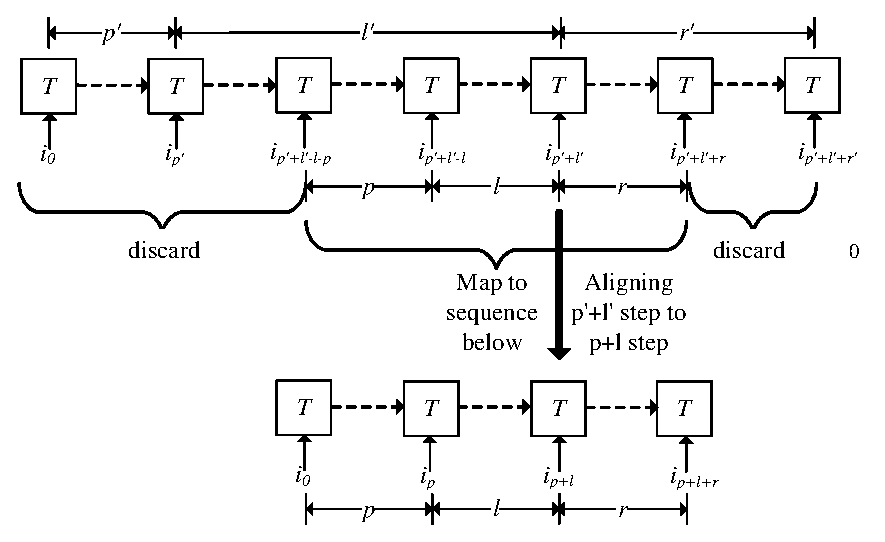
\includegraphics[width=0.7\textwidth]{pcmap}
\end{center}
\caption{Mapping $F'^d_{PC}(p',l',r',1)$ to $F'^d_{PC}(p,l,r,1)$ by aligning $(p'+l')$-step to $(p+l)$-step.}
  \label{fig_pcmap}
\end{figure}

\begin{figure}[b]
\begin{center}
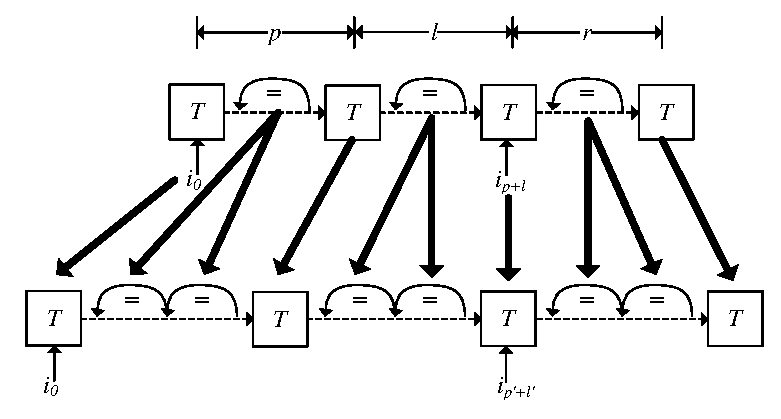
\includegraphics[width=0.7\textwidth]{lnmap}
\end{center}
\caption{Mapping $F'^d_{LN}(p,l,r,1)$ to $F'^d_{LN}(p',l',r',1)$ by aligning $(p+l)$-step to $(p'+l')$-step.}
  \label{fig_lnmap}
\end{figure}

\begin{lemma}\label{lemmalninc}
$\mathbf{FSAT_{LN}(p,l,r)}$ in Algorithm \ref{algo_infer} monotonically increases  with respect to $p$, $l$ and $r$.
\end{lemma}
\begin{proof}
For any $p'>p$,$l'>l$ and $r'>l$,
assume $A:\vec{f}_{p+l}\to B$ is a Boolean valuation of the flow control vector 
at $(p+l)$-step.
Further assume that $A$ is covered by $FSAT_{LN}(p,l,r)$.

So $A$ can make $F'^d_{LN}(p,l,r,1)$ satisfiable.
Assume this satisfying assignment of $F'^d_{LN}(p,l,r,1)$ is $A'$.
We know that $A(\vec{f}_{p+l})\equiv A'(\vec{f}_{p+l})$.

As shown in Figure \ref{fig_lnmap},
we can map $F'^d_{LN}(p,l,r,1)$ to $F'^d_{LN}(p',l',r',1)$ by aligning $(p+l)$-step to $(p'+l')$-step,
and unrolling those three loops.
In this way we can get another satisfying assignment $A''$ of $F'^d_{LN}(p',l',r',1)$.

By restricting the domain of $A''$ to $vec{f}_{p'+l'}$,
we can get the fourth satisfying assignment $A''':\vec{f}_{p'+l'}\to B$.
It is obvious that $A\equiv A'''$.

This means that every valuation covered by $FSAT_{LN}(p,l,r)$ is also covered by $FSAT_{LN}(p',l',r')$.
So $FSAT_{LN}(p,l,r)$ grow monotonically with respect to $p$, $l$ and $r$.
\end{proof}


\begin{lemma}\label{lemmaln2pc}
$FSAT_{LN}(p,l,r)\Rightarrow FSAT_{PC}(p,l,r)$
\end{lemma}
\begin{proof}
It is obvious that the clause set of $F'^d_{LN}(p,l,r,1)$ is a super set of $F'^d_{PC}(p,l,r,1)$.
So every satisfying assignment of $F'^d_{LN}(p,l,r,1)$ can also satisfy $F'^d_{PC}(p,l,r,1)$.
so $FSAT_{LN}(p,l,r)\Rightarrow FSAT_{PC}(p,l,r)$ holds.
\end{proof}

These three lemmas are depicted intuitively in Figure \ref{fig_mono},
which makes it obvious that $\neg FSAT_{LN}(p,l,r)\wedge FSAT_{PC}(p,l,r)$ monotonically decreases in Algorithm \ref{algo_infer}.
With these lemmas,
let's first prove that Algorithm \ref{algo_infer} is a halting one.

\begin{theorem}
 Algorithm \ref{algo_infer} is a halting algorithm.
\end{theorem}


\begin{proof}
As the encoder is represented by a finite state machine,
the length of the longest path without loop is finite.
If Algorithm \ref{algo_infer} does not halt,
then eventually the values of $p$, $l$ and $r$ in Algorithm \ref{algo_infer} will be larger than the length of the longest path without loop,
which means there will be loops in these three state sequences $<\vec{s}_{0},\dots,\vec{s}_{p}>$,$<\vec{s}_{p+1},\dots,\vec{s}_{p+l}>$ and 
$<\vec{s}_{p+l+1},\dots,\vec{s}_{p+l+r}>$.
Thus,
every satisfying assignment of $F'^d_{PC}(p,l,r,1)$ also satisfies $F'^d_{LN}(p,l,r,1)$,
which means $\neg FSAT_{LN}(p,l,r)\wedge FSAT_{PC}(p,l,r)$ is unsatisfiable.
This will lead to the termination of Algorithm \ref{algo_infer}.
So,
it is a halting algorithm.
\end{proof}



We will then prove the correctness of Algorithm \ref{algo_infer}.

\begin{theorem}
$\neg FSAT_{LN}(p,l,r)$ returned by Algorithm \ref{algo_infer} covers and only covers all valuations of $\vec{f}$ that
enable $\vec{d}$ to be uniquely determined by a bounded sequence of $\vec{o}$.
\end{theorem}
\begin{proof}
Let's first prove the covering case.
$FSAT_{LN}(p,l,r)$ covers a set of valuations of $\vec{f}$ that make 
$\vec{d}$ to be not uniquely determined for some particular $p$, $l$ and $r$.
So $\neg FSAT_{LN}(p,l,r)$ rules them out and covers all  valuations of $\vec{f}$ that
enable $\vec{d}$ to be uniquely determined.

We then prove the only covering case.
If $A$ is a valuation of $\vec{f}$ covered by $\neg FSAT_{LN}(p,l,r)$ that makes $\vec{d}$ to be \textbf{NOT} uniquely determined for some particular $p'$, $l'$ and $r'$,
then we have:

\begin{enumerate}
 \item $FSAT_{LN}(p',l',r')$ also covers $A$.
 According to Lemma \ref{lemmalninc},
 for all $p''>max(p',p)$,$l''>max(l',l)$ and $r''>max(r',r)$,
 $FSAT_{LN}(p'',l'',r'')$ also covers $A$.
 \item $FSAT_{LN}(p,l,r)$ does not cover $A$.
 It is the last $FSAT_{LN}(p,l,r)$ computed by Algorithm \ref{algo_infer}.
 Which means that the $valid(\vec{f})$'s under-approximation and over-approximation have converge.
 So for all $p''>max(p',p)$,$l''>max(l',l)$ and $r''>max(r',r)$,
 $FSAT_{LN}(p'',l'',r'')$ must be equal to $FSAT_{LN}(p,l,r)$.
 Thus $FSAT_{LN}(p'',l'',r'')$ also does not cover $A$.
\end{enumerate}

These two cases conflit with each other.
So there is no such $A$ covered by $\neg FSAT_{LN}(p,l,r)$ that makes $\vec{d}$ to be \textbf{NOT} uniquely determined for some particular $p'$, $l'$ and $r'$.
So the only covering case is proved.
\end{proof}


\section{Minimizing the valuation of $l$ and $r$}\label{sec_min}
We will first introduce why and how to remove the redundancy of $l$ and $r$ in Subsection \ref{reduceing},
and then present another possible structure of our algorithm in Subsection \ref{alter},
and discuss why we have chosen the one in Subsection \ref{reduceing} instead of the one in Subsection \ref{alter}.

\subsection{Minimizing the valuation of $l$ and $r$}\label{reduceing}
As we have increase the value of $p$,$l$ and $r$ simultaneously in Algorithm \ref{algo_infer},
there may be some redundancy in the valuation of $p$,$l$ and $r$,
which may lead to unnecessary overhead in the decoder's circuit area and delay.

For example,
assume the encoder is a simple buffer whose $o:=i$.
With $p\equiv 0$,$l\equiv 0$ and $r\equiv 0$,
we can get the simplest decoder $i:=o$.
In such a decoder,
there is only one buffer and no registers.
But with $p\equiv 0$,$l\equiv 0$ and $r\equiv 1$,
we need an additional register to delay $o$ for one step,
and then recover $i_i$ from the delayed $o$.

According to Figure \ref{fig_pc},
it is obvious that,
$r$ affect both the decoder's latency and circuit area,
$l$ affect only the decoder's circuit area,
while $p$ does not affect the decoder.

So as shown in Algorithm \ref{algo_remove2}
we chose to first minimize $r$, 
then minimize $l$.

\begin{algorithm}[t]
\SetAlgoVlined
\For{$r':=r \to 1$} {
  \If{$F_{PC}(p,l,r'-1)\wedge valid(\vec{f}_{p+l})$ is satisfiable} {
    break
  }
  \ElseIf{$r'\equiv 1$} {
    $r':=r'-1$\\
    break
  }
}
\For{$l':=l \to 1$} {
  \If{$F_{PC}(p,l'-1,r')\wedge valid(\vec{f}_{p+l'-1})$ is satisfiable} {
    break
  }
  \ElseIf{$l'\equiv 1$} {
    $l':=l'-1$\\
    break
  }
}
return $<l',r'>$
\caption{$RemoveRedundancy(p,l,r)$}
\label{algo_remove2}
\end{algorithm}

% To simply the presentation,
% we still use $p$, $l$ and $r$ instead of $p'$, $l'$ and $r'$ in the remainder of this paper.

\subsection{An alternative approach for comparison}\label{alter}

In above discussion,
we first find out the flow control variables by increasing $p$, $l$ and $r$ simultaneously in Algorithm \ref{alg_fofc_inc},
and then minimize their valuations with Algorithm \ref{algo_remove2}.
This approach need to call SAT solver for $O(n)$ times,
with $n=max(p,l,r)$.

\textbf{
There is another possible way to do this job in Algorithm \ref{alg_fofc_inc},
that is,
increasing $p$, $l$ and $r$ one by one with three nested loops,
instead of simultaneously.
This approach need to call SAT solver for $O(n^3)$ times,
}


\textbf{
We will show in Subsection \ref{subsec_incr_plr_exp} that,
increasing $p$, $l$ and $r$ simultaneously and then minimized them with Algorithm \ref{algo_remove2} is much faster than increasing them separately.
We will also explain the reason there.
}

\section{Characterizing the decoder's Boolean function}\label{sec_char}
In Section \ref{sec_findfc},
the encoder's input vector $\vec{i}$ has been partitioned into two vectors:
the flow control vector $\vec{f}$ and the data vector $\vec{d}$.
The algorithms to characterize the decoder's Boolean functions that compute $\vec{f}$ and $\vec{d}$ are different,
so they are discussed separately in the following two subsections.

\subsection{Characterizing the decoder's Boolean function that computes $\vec{f}$}\label{subsec_fdec}

Each variable $f\in \vec{f}$ can be uniquely determined by a bounded sequence of the encoder's output.
So,
for each particular valuation of the encoder's output sequence $<\vec{o}_p,\dots,\vec{o}_{p+l+r}>$,
$f_{p+l}$ cannot be 0 and 1 at the same time.
Thus,
the decoder's Boolean function that computes $f_{p+l}$ is exactly the Craig interpolant of $\phi_A$ with respect to $\phi_B$:

\begin{equation}\label{fa}
\phi_A:=
\left\{
\begin{array}{cc}
&\bigwedge_{m=0}^{p+l+r}
\{
(\vec{s}_{m+1},\vec{o}_m)\equiv T(\vec{s}_m,\vec{i}_m)
\}
\\
\wedge& f_{p+l}\equiv 1 \\
\wedge&\bigwedge_{m=0}^{p+l+r}assertion(\vec{i}_m) 
\end{array}
\right\}
\end{equation}

\begin{equation}\label{fb}
\phi_B:=
\left\{
\begin{array}{cc}
&\bigwedge_{m=0}^{p+l+r}
\{
(\vec{s'}_{m+1},\vec{o'}_m)\equiv T(\vec{s'}_m,\vec{i'}_m)
\}
\\
\wedge&\bigwedge_{m=p}^{p+l+r}\vec{o}_m\equiv \vec{o'}_m \\
\wedge& f'_{p+l}\equiv 0 \\
\wedge&\bigwedge_{m=0}^{p+l+r}assertion(\vec{i'}_m) 
\end{array}
\right\}
\end{equation}

It is obvious that $\phi_A\wedge \phi_B$ equals $F_{PC}(p,l,r)$ in Equation (\ref{uniqt1}),
so it is unsatisfiable.
The common variable set of $\phi_A$ and $\phi_B$ is $<\vec{o}_p,\dots,\vec{o}_{p+l+r}>$.
So,
a Craig interpolant $ITP$ can be derived by McMillian's algorithm\cite{interp_McMillan} from the unsatisfiability proof of $\phi_A\wedge \phi_B$,
which covers all values of $<\vec{o}_p,\dots,\vec{o}_{p+l+r}>$ that make $f_{p+l}\equiv 1$.
At the same time,
$ITP\wedge \phi_B$ is unsatisfiable,
so $ITP$ covers nothing that can make $f_{p+l}\equiv 0$.
Thus,
$ITP$ is the decoder's Boolean function that computes $f\in\vec{f}$.

To speedup characterizing the decoder's Boolean function for all $f\in\vec{f}$,
we can employ the incremental SAT mechanism in MiniSat again by:
\begin{enumerate}
 \item 
 Removing $f_{p+l}\equiv 1$ from $\phi_A$ and $f'_{p+l}\equiv 0$ from $\phi_B$.
 \item 
 Adding $\phi_A\wedge \phi_B$ into the MiniSat's clause database.
 \item 
 Solving with assumptions $f_{p+l}\equiv 1$ and $f'_{p+l}\equiv 0$ for each $f\in\vec{f}$.
 And generating Craig interpolants separately.
\end{enumerate}

\subsection{Characterizing the decoder's Boolean function that computes $\vec{d}$}

Assume that the predicate over $\vec{f}$ inferred by Algorithm \ref{algo_infer},
is $valid(\vec{f})$.
Let's define the following two formulas for each data variable $d\in\vec{d}$:

\begin{equation}\label{da}
\phi_A':=
\left\{
\begin{array}{cc}
&\bigwedge_{m=0}^{p+l+r}
\{
(\vec{s}_{m+1},\vec{o}_m)\equiv T(\vec{s}_m,\vec{i}_m)
\}
\\
\wedge& d_{p+l}\equiv 1 \\
\wedge& valid(\vec{f}_{p+l}) \\
\wedge&\bigwedge_{m=0}^{p+l+r}assertion(\vec{i}_m) 
\end{array}
\right\}
\end{equation}

\begin{equation}\label{db}
\phi_B':=
\left\{
\begin{array}{cc}
&\bigwedge_{m=0}^{p+l+r}
\{
(\vec{s'}_{m+1},\vec{o'}_m)\equiv T(\vec{s'}_m,\vec{i'}_m)
\}
\\
\wedge&\bigwedge_{m=p}^{p+l+r}\vec{o}_m\equiv \vec{o'}_m \\
\wedge& d'_{p+l}\equiv 0\\
\wedge& valid(\vec{f'}_{p+l})\\
\wedge&\bigwedge_{m=0}^{p+l+r}assertion(\vec{i'}_m) 
\end{array}
\right\}
\end{equation}

Each variable $d\in \vec{d}$ can be uniquely determined by the encoder's output only when $valid(\vec{f})$ holds.
So,
if $valid(\vec{f}_{p+l})$ holds,
for each particular valuation of the encoder's output sequence $<\vec{o}_p,\dots,\vec{o}_{p+l+r}>$,
$d_{p+l}$ cannot be 0 and 1 at the same time.
So,
$\phi_A'\wedge \phi_B'$ is unsatisfiable.
Thus,
a Craig interpolant $ITP$ can be derived by McMillian's algorithm\cite{interp_McMillan} from the unsatisfiability proof of $\phi_A'\wedge \phi_B'$,
which covers and only covers all valuations of $<\vec{o}_p,\dots,\vec{o}_{p+l+r}>$ that make $d_{p+l}\equiv 1$.
Thus,
$ITP$ is the decoder's Boolean function that computes $d\in\vec{d}$.

Furthermore,
when $valid(\vec{f}_{p+l})$ does not hold,
the data variable $d\in\vec{d}_{p+l}$ cannot be uniquely determined.
So,
no function can be used to calculate its value.
But this is not a problem,
because the decoder is supposed 
to only recover the value of control flow vector $\vec{f}$,
and ignore the exact value of $\vec{d}$ in this case.

Similarly,
we can also use the incremental SAT approach in Subsection \ref{subsec_fdec} to speedup characterizing the decoder's Boolean function for all $d\in\vec{d}$.


% 
% As a new technology, Wireless Sensor Networks (WSNs) has a wide
% range of applications [Culler 2001,Bahl 2002,Akyildiz 2001], including
% environment monitoring, smart buildings, medical care, industrial and
% military applications. Among them, a recent trend is to develop
% commercial sensor networks that require pervasive sensing of both
% environment and human beings, for example, assisted living
% [Akyildiz 2002,Harvard 2001,CROSSBOW] and smart homes
% [Harvard 2001,Adya 2001,CROSSBOW].
% % quote
% \begin{quote}
% ``For these applications, sensor devices are incorporated into human
% cloths [Natarajan 2001,Zhou 2006,Bahl 2002,Adya 2001] for monitoring
% health related information like EKG readings, fall detection, and voice recognition".
% \end{quote}
% While collecting all these multimedia information
% [Akyildiz 2002] requires a high network throughput, off-the-shelf
% sensor devices only provide very limited bandwidth in a single
% channel: 19.2Kbps in MICA2 [Bahl 2002] and 250Kbps in MICAz.
% 
% In this article, we propose MMSN, abbreviation for Multifrequency
% Media access control for wireless Sensor Networks. The main
% contributions of this work can be summarized as follows.
% % itemize
% \begin{itemize}
% \item To the best of our knowledge, the MMSN protocol is the first
% multifrequency MAC protocol especially designed for WSNs, in which
% each device is equipped with a single radio transceiver and
% the MAC layer packet size is very small.
% \item Instead of using pairwise RTS/CTS frequency negotiation
% [Adya 2001,Culler 2001; Tzamaloukas 2001; Zhou 2006],
% we propose lightweight frequency assignments, which are good choices
% for many deployed comparatively static WSNs.
% \item We develop new toggle transmission and snooping techniques to
% enable a single radio transceiver in a sensor device to achieve
% scalable performance, avoiding the nonscalable ``one
% control channel + multiple data channels'' design [Natarajan 2001].
% \end{itemize}

% Head 1
% \section{MMSN Protocol}
% 
% % Head 2
% \subsection{Frequency Assignment}
% 
% We propose a suboptimal distribution to be used by each node, which is
% easy to compute and does not depend on the number of competing
% nodes. A natural candidate is an increasing geometric sequence, in

% which
% % Numbered Equation
% \begin{equation}
% \label{eqn:01}
% P(t)=\frac{b^{\frac{t+1}{T+1}}-b^{\frac{t}{T+1}}}{b-1},
% \end{equation}
% where $t=0,{\ldots}\,,T$, and $b$ is a number greater than $1$.
% 
% In our algorithm, we use the suboptimal approach for simplicity and
% generality. We need to make the distribution of the selected back-off
% time slice at each node conform to what is shown in Equation
% (\ref{eqn:01}). It is implemented as follows: First, a random
% variable $\alpha$ with a uniform distribution within the interval
% $(0, 1)$ is generated on each node, then time slice $i$ is selected
% according to the following equation:
% % Unnumbered Equation
% \[
% i=\lfloor(T+1)\log_b[\alpha(b-1)+1]\rfloor.
% \]
% It can be easily proven that the distribution of $i$ conforms to Equation
% (\ref{eqn:01}).
% 
% So protocols [Bahl 2002,Culler 2001,Zhou 2006,Adya 2001,Culler 2001;
% Tzamaloukas-01; Akyildiz-01] that use RTS/CTS
% controls\footnote{RTS/CTS controls are required to be implemented by
% 802.11-compliant devices. They can be used as an optional mechanism
% to avoid Hidden Terminal Problems in the 802.11 standard and
% protocols based on those similar to [Akyildiz 2001] and
% [Adya 2001].} for frequency negotiation and reservation are not
% suitable for WSN applications, even though they exhibit good
% performance in general wireless ad hoc
% networks.
% 
% % Head 3
% \subsubsection{Exclusive Frequency Assignment}
% 
% In exclusive frequency assignment, nodes first exchange their IDs
% among two communication hops so that each node knows its two-hop
% neighbors' IDs. In the second broadcast, each node beacons all
% neighbors' IDs it has collected during the first broadcast period.
% 
% % Head 4
% \paragraph{Eavesdropping}
% 
% Even though the even selection scheme leads to even sharing of
% available frequencies among any two-hop neighborhood, it involves a
% number of two-hop broadcasts. To reduce the communication cost, we
% propose a lightweight eavesdropping scheme.
% 
% \subsection{Basic Notations}
% 
% As Algorithm~\ref{alg:one} states, for each frequency
% number, each node calculates a random number (${\textit{Rnd}}_{\alpha}$) for
% itself and a random number (${\textit{Rnd}}_{\beta}$) for each of its two-hop
% neighbors with the same pseudorandom number generator.
% % Algorithm
% \begin{algorithm}[t]
% \SetAlgoNoLine
% \KwIn{Node $\alpha$'s ID ($ID_{\alpha}$), and node $\alpha$'s
% neighbors' IDs within two communication hops.}
% \KwOut{The frequency number ($FreNum_{\alpha}$) node $\alpha$ gets assigned.}
% $index$ = 0; $FreNum_{\alpha}$ = -1\;
% \Repeat{$FreNum_{\alpha} > -1$}{
%         $Rnd_{\alpha}$ = Random($ID_{\alpha}$, $index$)\;
%         $Found$ = $TRUE$\;
%         \For{each node $\beta$ in $\alpha$'s two communication hops
%     }{
%       $Rnd_{\beta}$ = Random($ID_{\beta}$, $index$)\;
%       \If{($Rnd_{\alpha} < Rnd_{\beta}$) \text{or} ($Rnd_{\alpha}$ ==
%           $Rnd_{\beta}$ \text{and} $ID_{\alpha} < ID_{\beta}$)\;
%       }{
%         $Found$ = $FALSE$; break\;
%       }
%         }
%      \eIf{$Found$}{
%            $FreNum_{\alpha}$ = $index$\;
%          }{
%            $index$ ++\;
%      }
%       }
% \caption{Frequency Number Computation}
% \label{alg:one}
% \end{algorithm}
% 
% Bus masters are divided into two disjoint sets, $\mathcal{M}_{RT}$
% and $\mathcal{M}_{NRT}$.
% % description
% \begin{description}
% \item[RT Masters]
% $\mathcal{M}_{RT}=\{ \vec{m}_{1},\dots,\vec{m}_{n}\}$ denotes the
% $n$ RT masters issuing real-time constrained requests. To model the
% current request issued by an $\vec{m}_{i}$ in $\mathcal{M}_{RT}$,
% three parameters---the recurrence time $(r_i)$, the service cycle
% $(c_i)$, and the relative deadline $(d_i)$---are used, with their
% relationships.
% \item[NRT Masters]
% $\mathcal{M}_{NRT}=\{ \vec{m}_{n+1},\dots,\vec{m}_{n+m}\}$ is a set
% of $m$ masters issuing nonreal-time constrained requests. In our
% model, each $\vec{m}_{j}$ in $\mathcal{M}_{NRT}$ needs only one
% parameter, the service cycle, to model the current request it
% issues.
% \end{description}
% 
% Here, a question may arise, since each node has a global ID. Why
% don't we just map nodes' IDs within two hops into a group of
% frequency numbers and assign those numbers to all nodes within two
% hops?
% 
% \section{Simulator}
% \label{sec:sim}
% 
% If the model checker requests successors of a state which are not
% created yet, the state space uses the simulator to create the
% successors on-the-fly. To create successor states the simulator
% conducts the following steps.
% % enumerate
% \begin{enumerate}
% \item Load state into microcontroller model.
% \item Determine assignments needed for resolving nondeterminism.
% \item For each assignment.
%       \begin{enumerate}
%       \item either call interrupt handler or simulate effect of next instruction, or
%       \item evaluate truth values of atomic propositions.
%       \end{enumerate}
% \item Return resulting states.
% \end{enumerate}
% Figure~\ref{fig:one} shows a typical microcontroller C program that
% controls an automotive power window lift. The program is one of the
% programs used in the case study described in Section~\ref{sec:sim}.
% At first sight, the programs looks like an ANSI~C program. It
% contains function calls, assignments, if clauses, and while loops.
% % Figure
% \begin{figure}
% \centerline{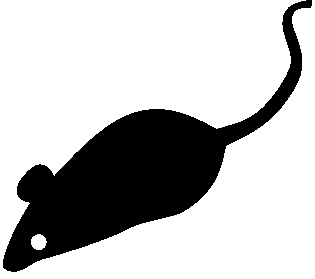
\includegraphics{acmsmall-mouse}}
% \caption{Code before preprocessing.}
% \label{fig:one}
% \end{figure}
% 
% \subsection{Problem Formulation}
% 
% The objective of variable coalescence-based offset assignment is to find
% both the coalescence scheme and the MWPC on the coalesced graph. We start
% with a few definitions and lemmas for variable coalescence.
% 
% % Enunciations
% \begin{definition}[Coalesced Node (C-Node)]A C-node is a set of
% live ranges (webs) in the AG or IG that are coalesced. Nodes within the same
% C-node cannot interfere with each other on the IG. Before any coalescing is
% done, each live range is a C-node by itself.
% \end{definition}
% 
% \begin{definition}[C-AG (Coalesced Access Graph)]The C-AG is the access
% graph after node coalescence, which is composed of all C-nodes and C-edges.
% \end{definition}
% 
% \begin{lemma}
% The C-MWPC problem is NP-complete.
% \end{lemma}
% \begin{proof} C-MWPC can be easily reduced to the MWPC problem assuming a
% coalescence graph without any edge or a fully connected interference graph.
% Therefore, each C-node is an uncoalesced live range after value separation
% and C-PC is equivalent to PC. A fully connected interference graph is made
% possible when all live ranges interfere with each other. Thus, the C-MWPC
% problem is NP-complete.
% \end{proof}
% 
% \begin{lemma}[Lemma Subhead]The solution to the C-MWPC problem is no
% worse than the solution to the MWPC.
% \end{lemma}
% \begin{proof}
% Simply, any solution to the MWPC is also a solution to the
% C-MWPC. But some solutions to C-MWPC may not apply to the MWPC (if any
% coalescing were made).
% \end{proof}
% 
% \section{Performance Evaluation}
% 
% During all the experiments, the Geographic Forwarding (GF)
% [Akyildiz 2001] routing protocol is used. GF exploits geographic
% information of nodes and conducts local data-forwarding to achieve
% end-to-end routing. Our simulation is
% configured according to the settings in
% Table~\ref{tab:one}. Each run lasts for 2 minutes and
% repeated 100 times. For each data value we present in the results,
% we also give its 90\% confidence interval.
% % Table
% \begin{table}%
% \tbl{Simulation Configuration\label{tab:one}}{%
% \begin{tabular}{|l|l|}
% \hline
% TERRAIN{$^a$}   & (200m$\times$200m) Square\\\hline
% Node Number     & 289\\\hline
% Node Placement  & Uniform\\\hline
% Application     & Many-to-Many/Gossip CBR Streams\\\hline
% Payload Size    & 32 bytes\\\hline
% Routing Layer   & GF\\\hline
% MAC Layer       & CSMA/MMSN\\\hline
% Radio Layer     & RADIO-ACCNOISE\\\hline
% Radio Bandwidth & 250Kbps\\\hline
% Radio Range     & 20m--45m\\\hline
% \end{tabular}}
% \begin{tabnote}%
% \Note{Source:}{This is a table
% sourcenote. This is a table sourcenote. This is a table
% sourcenote.}
% \vskip2pt
% \Note{Note:}{This is a table footnote.}
% \tabnoteentry{$^a$}{This is a table footnote. This is a
% table footnote. This is a table footnote.}
% \end{tabnote}%
% \end{table}%

\section{Experimental Results}\label{sec_exp}

We have implemented these algorithms in OCaml language,
and solved the generated CNF formulas with MiniSat 1.14\cite{EXTSAT}.
All experiments have been run on a server with 16 Intel Xeon E5648 processors at 2.67GHz, 
192GB memory, and CentOS 5.4 Linux.
All these experimental results and programs can be downloaded 
from https://github.com/shengyushen/compsyn.

\subsection{Benchmarks}
Table \ref{tab:summ} shows all benchmarks used in this paper.
They come from two sources:
\begin{enumerate}
 \item Our previous paper \cite{ShenTCAD12}. 
 \item \cite{LiuTCAD12}.
%  \item The benchmark package sent to us by Liu, the author of \cite{LiuTCAD12}.
%  So there may be some overlap between (2) and (3).
\end{enumerate}

Each column of Table \ref{tab:summ} shows respectively the number of input, output and register of each benchmarks.
The \#gate and area columns show the number of gates and area of the encoder when mapped to mcnc.genlib library by
ABC synthesis tool \cite{ABC} with script "strash; dsd; strash; dc2; dc2; dch; map".
In the remainder of this paper, 
all circuit areas, gate number and delay are obtained in the same setting such that we can compare them to that of \cite{LiuTCAD12}.

\begin{table}[b]%
\tbl{Benchmarks\label{tab:summ}}{%
\begin{tabular}{|c|c|c|c|c|c|c|}
\hline
                 & Names     &    \#     &      \#     &Circuit& Description                         & How to                     \\
                 &           & in/out    &  reg/gate   &area  &   of Encoders                        & handle                     \\\hline\hline
                 & PCIE2     & 10 / 11   & 22   / 149  & 326  &PCIE 2.0                              & Subsection                 \\
Benchmarks       &           &           &             &      &\cite{pcie21}                         & \ref{subsec_pcie2}         \\\cline{2-7}
 in Shen         & XGXS      & 10 / 10   & 17   / 249  & 572  &10Gb Ethernet in clause               & Subsection                 \\
\citeyear{ShenTCAD12} with&  &           &             &      & 48 of \cite{IEEE8023_S4}             & \ref{subsec_10g}           \\\cline{2-7}
flow control     & T2Eth     & 14 / 14   & 53   / 427  & 947  &Ethernet encoder of                   & Subsection                 \\
                 &           &           &             &      &UltraSPARC T2 processor               &\ref{subsec_t2e}            \\\hline\hline
Benchmarks       & XFI       & 72 / 66   & 72   / 5086 & 12381&10Gb Ethernet in clause               &                            \\
 in Shen         &           &           &             &      & 49 of \cite{IEEE8023_S4}             &Comparing                   \\\cline{2-6}
\citeyear{ShenTCAD12} without&SCRAMBLER&64/64&58/353   & 1034 & Making a bit stream to               &our                         \\
flow control     &           &           &             &      & have lots of 01 flipping             & algorithm                  \\\cline{1-6}
                 & CC\_3     &   1/3     &   6/22      & 54   &convolution code                      &to Liu\citeyear{LiuTCAD12}  \\
                 &           &           &             &      & with length 3                        &in                          \\\cline{2-6}  
                 & CC\_4     &   1/3     &   7/26      & 63   &convolution code                      &Subsection                  \\
Benchmarks       &           &           &             &      &with length 4                         &\ref{subsec_nonflow}        \\\cline{2-6}
in \cite{LiuTCAD12}&HM(7,4)  &   4/7     &   3/38      &  103 & Hamming encoder                      &                            \\
                 &           &           &             &      & with 4 inputs and 7 outputs          &                            \\\cline{2-6}
                 &HM(15,11)  &   11/15   &   4/102     & 317  & Hamming encoder                      &                            \\
                 &           &           &             &      & with 11 inputs and 15 outputs        &                            \\\hline
\end{tabular}}
\end{table}%

The last column of Table \ref{tab:summ} also shows 
how will we present the experimental result of these benchmarks:
\begin{enumerate}
 \item 
By studying the 5 benchmarks used in our previous papers \cite{ShenTCAD12},
we found that most of them have built-in flow control mechanisms.
This is not a surprise to us,
because these benchmarks all come from real industrial projects.
These three benchmarks will be presented in Subsection 
\ref{subsec_pcie2},\ref{subsec_10g} and \ref{subsec_t2e}.
 \item 
For all other benchmarks in Table \ref{tab:summ} without flow control mechanism,
if their input variables can always uniquely determined,
our algorithm can recognize all their input variables as flow control variables,
and direct generate their decoder's Boolean functions.
Their experimental results will be presented in Subsection \ref{subsec_nonflow}.
%  \item 
% The last two benchmarks in Table \ref{tab:summ} only exist in \cite{LiuTCAD12}.
% We can not find their source code in the benchmark package sent to us by Liu.
% So we will not discuss them here.
\end{enumerate}

We have also conducted other experiments:

In Subsection \ref{subsec_incr_plr_exp}, we will compare run time overhead of two different approaches:
\begin{enumerate}
 \item Increasing $p$, $l$ and $r$ simultaneously in Algorithm \ref{algo_infer} 
 and then minimize them in Algorithm \ref{algo_remove2}.
 \item Increasing $p$, $l$ and $r$ separately with three nested loops in Algorithm \ref{algo_infer}.
\end{enumerate}

In Subsection \ref{subsec_min},
we will compare run times, circuit areas and delay between the two approaches 
that do and do not minimize $p$,$l$ and $r$ by Algorithm \ref{algo_remove2}.

Finally in Subsection \ref{subsec_compareman},
we will compare the circuit area and delay between the decoder generated by our algorithm with the decoder written manually.


\subsection{PCI Express 2.0 encoder}\label{subsec_pcie2}
This encoder is compliant with the PCI Express 2.0 standard \cite{pcie21}.
After deleting empty line and comments,
its source code has 259 lines of verilog.

\begin{table}[b]%
\tbl{The input and output variables of the PCI Express 2.0 encoder\label{tab:pcieio}}{%
\begin{tabular}{|c|c|c|c|}
\hline
         & variable name        & width & description\\\hline\hline
         & $TXDATA$             & 8     &The data to be encoded \\\cline{2-4}
Inputs   & $TXDATAK$            & 1     &1 means $TXDATA$ is a controlling character, \\
         &                      &       &0 means $TXDATA$ is normal data \\\cline{2-4}
         & $CNTL\_TXEnable\_P0$ & 1     &Indicating the validness of $TXDATA$ and $TXDATAK$\\\hline
Outputs  & $HSS\_TXD$           & 10    &The encoded data \\\cline{2-4}
         & $HSS\_TXELECIDLE$    & 1     &The electrical idle state\\\hline
\end{tabular}}
\end{table}%

The list of input and output variables is shown in Table \ref{tab:pcieio}.
According to the 8b/10b encoding scheme's coding table\cite{encode8b10b},
when $TXDATAK\equiv 0$,
$TXDATA$ can be of any value.
But when $TXDATAK\equiv 1$,
$TXDATA$ can only be 1C, 3C, 5C, 7C, 9C, BC, DC, FC, F7, FB, FD and FE.
So,
we write an assertion to rule out those combinations that are not in this coding table.
This assertion is embed into the transition function $T$,
so that it can be enforced at every step in the unrolled state sequences.

Algorithm \ref{alg_fofc} identifies the flow control variable $\vec{f}:=CNTL\_TXEnable\_P0$ in 0.475 seconds.
And then Algorithm \ref{algo_infer} infers the predicate $valid(\vec{f}):=CNTL\_TXEnable\_P0$ 
that enables the data vector to be uniquely determined in 1.22 seconds.
And then Algorithm \ref{algo_remove2} obtains the minimized $p:=4$, $l:=0$ and $r:=2$ in 0.69 seconds.
Finally, 
with the inferred $valid(\vec{f})$,
generating the decoder's Boolean functions for $CNTL\_TXEnable\_P0$, $TXDATA$ and $TXDATAK$ costs 0.26 seconds.
The decoder contains 156 gates and 0 registers with area 366 and delay 7.6.


The major breakthrough of this paper's algorithms is their ability to handle invalid data vector.
So,
it should be very interesting to show how the invalid data vector is mapped to output variable vector $\vec{o}$.
By studying the source code of this encoder,
we find that,
when and only when $CNTL\_TXEnable\_P0\equiv 0$ holds,
that is,
$TXDATA$ and $TXDATAK$ are invalid,
the output electrical idle variable $HSS\_TXELECIDLE$ becomes 1.
% which will force the analog transmitter into a electrical idle state.
% The analog receiver can detect such an electrical idle state and recover the $HSS\_TXELECIDLE$.
So,
the decoder can use the output variable $HSS\_TXELECIDLE$ to uniquely determine the value of flow control variable $CNTL\_TXEnable\_P0$.

\begin{table}[t]%
\tbl{The input and output variables of the 10G Ethernet encoder XGXS\label{tab:eth10g}}{%
\begin{tabular}{|c|c|c|c|}
\hline
         & variable name          & width & description\\\hline\hline
         & $encode\_data\_in$   & 8     &The data to be encoded \\\cline{2-4}
Inputs   & $konstant$           & 1     &1 means $encode\_data\_in$ is a special character, \\
         &                      &       &0 means $encode\_data\_in$ is normal data \\\cline{2-4}
         & $bad\_code$          & 1     &Indicating the validness of $konstant$ and $encode\_data\_in$\\\hline
Outputs  & $encode\_data\_out$  & 10    &The encoded data \\\hline
\end{tabular}}
% \begin{tabnote}%
% \Note{Source:}{This is a table
% sourcenote. This is a table sourcenote. This is a table
% sourcenote.}
% \vskip2pt
% \Note{Note:}{This is a table footnote.}
% \tabnoteentry{$^a$}{This is a table footnote. This is a
% table footnote. This is a table footnote.}
% \end{tabnote}%
\end{table}%

\subsection{10G Ethernet encoder XGXS}\label{subsec_10g}
This encoder XGXS is compliant with clause 48 of IEEE 802.3 standard \cite{IEEE8023_S4}.
After deleting empty line and comments,
this encoder has 214 lines of verilog.

The list of input and output variables is shown in Table \ref{tab:eth10g}.
This encoder also employs an 8b/10b encoding scheme\cite{encode8b10b} with two inputs:
the 8-bit $encode\_data\_in$ to be encoded
and 1-bit $konstant$ indicating a controlling character.
According to the coding table in \cite{encode8b10b},
when $konstant\equiv 0$,
$encode\_data\_in$ can be of any value.
But when $konstant\equiv 1$,
$encode\_data\_in$ can only be 1C, 3C, 5C, 7C, 9C, BC, DC, FC, F7, FB, FD and FE.
So,
we write an assertion to exclude those combinations that are not in this table
and embed it into the the transition function $T$.

Algorithm \ref{alg_fofc} identifies the flow control variable $\vec{f}:=bad\_code$ in 0.31 seconds.
And then Algorithm \ref{algo_infer} infers the predicate $valid(\vec{f}):=\!bad\_code$ 
that enables the data vector to be uniquely determined in 0.95 seconds.
And then Algorithm \ref{algo_remove2} obtains the minimized $p:=4$, $l:=0$ and $r:=1$ in 0.52 seconds.
Finally, generating the decoder's Boolean functions for $bad\_code$, $encode\_data\_in$ and $konstant$ costs 0.17 seconds.
The decoder contains 163 gates and 0 registers with area 370 and delay 8.1.

Although this encoder uses the same coding mechanism as does the PCI Express 2.0 encoder mentioned above,
the way it handles the invalid data vector is different.
This encoder does not have a separate output variable to indicate the validness of the output data;
instead,
the validness and exact value of all input variables are both encoded in $encode\_data\_out$.
By studying this encoder's source code,
we find that when and only when $bad\_code\equiv 1$,
that is,
$encode\_data\_in$ and $konstant$ are invalid,
the output variable $encode\_data\_out$ will become  $0010111101$.
So the decoder can use the output variable $encode\_data\_out$ to uniquely determine the value of the flow control variable $bad\_code$.



\subsection{UltraSPARC T2 Ethernet encoder}\label{subsec_t2e}
This encoder comes from the UltraSPARC T2 open source processor designed by Sun Microsystems.
It is compliant with clause 36 of IEEE 802.3 standard \cite{IEEE8023_S4}.
After deleting empty line and comments,
this encoder's source code has 864 lines of verilog.


\begin{table}[b]%
\tbl{The input and output variables of the UltraSPARC T2 Ethernet encoder\label{tab:t2eth}}{%
\begin{tabular}{|c|c|c|c|}
\hline
         & variable name          & width & description\\\hline\hline
         & $txd$                & 8     &The data to be encoded \\\cline{2-4}
Inputs   & $tx\_enc\_ctrl\_sel$ & 1     &Refer to Table \ref{tab:one} \\\cline{2-4}
         & $tx\_en$             & 1     &Transmission enable \\\cline{2-4}
         & $tx\_er$             & 1     &Transmitting an error character \\\hline
         & $tx\_10bdata$        & 10    &The encoded data \\\cline{2-4}
         & $txd\_eq\_crs\_ext$  & 10    &Transmitting an special error character \\
Outputs  &                      &       &with $tx\_er\equiv 1$ and $txd\equiv 8'h0F$ \\\cline{2-4}
         & $tx\_er\_d$          & 1     &Transmitting an error character \\\cline{2-4}
         & $tx\_en\_d$          & 1     &Transmission enable \\\cline{2-4}
         & $pos\_disp\_tx\_p$   & 1     &Indicating positive parity \\\hline
\end{tabular}}
% \begin{tabnote}%
% \Note{Source:}{This is a table
% sourcenote. This is a table sourcenote. This is a table
% sourcenote.}
% \vskip2pt
% \Note{Note:}{This is a table footnote.}
% \tabnoteentry{$^a$}{This is a table footnote. This is a
% table footnote. This is a table footnote.}
% \end{tabnote}%
\end{table}%

The list of input and output variables is shown in Table \ref{tab:t2eth}.
This encoder also employs an 8b/10b encoding scheme\cite{encode8b10b},
but with yet another style of flow control mechanism that is significantly different from that of the above two encoders.
The data to be encoded is the 8-bit $txd$,
but there is no standalone variable to indicate the control symbol.
But only a 4-bit $tx\_enc\_ctrl\_sel$ used to define the action to be performed,
as shown in Table \ref{tab:one}.
It is obvious that the functionalities of the control symbol indication and flow control mechanism are combined in $tx\_enc\_ctrl\_sel$.
The last four cases in Table \ref{tab:one} can never be uniquely determined,
because they cannot be distinguished from the case of `PCS\_ENC\_DATA.
So we write an assertion to rule them out.

\begin{table}[t]%
\tbl{Actions to be performed in UltraSPARC T2 Ethernet encoder\label{tab:one}}{%
\begin{tabular}{|l|l|}
\hline
The name of action   & The meaning of action\\\hline\hline
`PCS\_ENC\_K285   & sending K28.5 control symbol\\\hline
`PCS\_ENC\_SOP  & sending K27.7 control symbol\\\hline
`PCS\_ENC\_T\_CHAR    & sending K29.7 control symbol\\\hline
`PCS\_ENC\_R\_CHAR   & sending K23.7 control symbol\\\hline
`PCS\_ENC\_H\_CHAR     & sending K30.7 control symbol\\\hline
`PCS\_ENC\_DATA     & sending the encoded txd\\\hline
`PCS\_ENC\_IDLE2     & sending D16.2 data symbol following K28.5\\\hline
`PCS\_ENC\_IDLE1       & sending D5.6 data symbol\\\hline
`PCS\_ENC\_LINK\_CONFA & sending D21.5 data symbol following K28.5\\\hline
`PCS\_ENC\_LINK\_CONFB     & sending D2.2 data symbol following K28.5\\\hline
\end{tabular}}
% \begin{tabnote}%
% \Note{Source:}{This is a table
% sourcenote. This is a table sourcenote. This is a table
% sourcenote.}
% \vskip2pt
% \Note{Note:}{This is a table footnote.}
% \tabnoteentry{$^a$}{This is a table footnote. This is a
% table footnote. This is a table footnote.}
% \end{tabnote}%
\end{table}%

Algorithm \ref{alg_fofc} identifies the flow control variables $\vec{f}:=\{tx\_enc\_ctrl\_sel,tx\_en, tx\_er\}$ in 3.76 seconds.
And then Algorithm \ref{algo_infer} infers the predicate $valid(\vec{f}):=tx\_enc\_ctrl\_sel\equiv `PCS\_ENC\_DATA$ 
that enables the data vector to be uniquely determined in 21.53 seconds.
And then Algorithm \ref{algo_remove2} obtains the minimized $p:=5$,$l:=0$ and $r:=4$ in 6.15 seconds.
Finally, generating the decoder's Boolean functions for $txd$, $tx\_enc\_ctrl\_sel$, $tx\_en$ and $tx\_er$ costs 3.40 seconds.
The decoder contains 401 gates and 9 registers with area 920 and delay 10.2.

As shown in the last column of Table \ref{tab:one},
the first 5 cases have their own particular control symbol values assigned to $tx\_10bdata$,
so the decoder can recover the value of the flow control variable $tx\_enc\_ctrl\_sel$ from $tx\_10bdata$.

\subsection{Comparing our algorithm with the state-of-the-art algorithm on circuits without flow control mechanism}\label{subsec_nonflow}

\begin{table}[b]%
\tbl{Comparing our algorithm with \cite{LiuTCAD12}\label{tab:comp_nocf}}{%
\begin{tabular}{|c|c|c|c|c|c|c|c|}
\hline
            &\multicolumn{4}{|c|}{Our algorithm}                    &\multicolumn{3}{|c|}{\cite{LiuTCAD12}}\\\cline{2-8}
            &time check.& time    & decoder & decoder               &time check. decoder & decoder & decoder               \\
Names       & decoder.  & gen.    & area    & delay                 & exist. and gen.    & area    & delay                 \\
            & exist.    & decoder &         &                       & decoder            &         &                       \\\hline
 PCIE2      &\multicolumn{7}{|c|}{} \\\cline{1-1}
 XGXS       &\multicolumn{7}{|c|}{Already presented in Subsection \ref{subsec_pcie2},\ref{subsec_10g} and \ref{subsec_t2e}.} \\\cline{1-1}
 T2Eth      &\multicolumn{7}{|c|}{} \\\hline
XFI         & 13.24     &6.13     & 3878    & 13.8                  & 8.59               &   3913  & 12.5\\\hline
SCRAMBLER   & 1.80      &0.55     & 698     & 3.8                   & 0.42               &   640   & 3.8 \\\hline
 CC\_3      &           &         & 128     & 8.5                   & 0.21               &   104   & 9.1 \\\hline
 CC\_4      &           &         & 490     & 13.3                  & 0.20               &   129   & 9.0 \\\hline
 HM(7,4)    & 0.09      &  0.03   & 258     & 8.1                   &   0.05             &   255   & 7.3 \\\hline
 HM(15,11)  &           &         & 5277    & 13.7                  &   2.02             &   3279  & 13.2\\\hline
\end{tabular}}
\end{table}%

Table \ref{tab:comp_nocf} compares our algorithm to \cite{LiuTCAD12} 
on those benchmarks without flow control mechanism.

The first 3 benchmarks have flow control mechanism and have been discussed in Subsection \ref{subsec_pcie2},\ref{subsec_10g} and \ref{subsec_t2e}.
So they are not discussed in this subsection.

For the 6 benchmarks from  XFI to HM(15,11),
we have their source code.
And \cite{LiuTCAD12} have its experimental result.
So we can compare the result of our algorithm to that of \cite{LiuTCAD12}.

By comparing the sum of the 2nd and 3rd columns to the 6th column,
we can find that \cite{LiuTCAD12} is much faster than our algorithm,
especially for the 2nd column.
I think this is caused by the fact that our algorithm need to spend lots of time 
to check whether each input variables $i\in \vec{i}$ can be uniquely determined,
while \cite{LiuTCAD12} can check all input variables with one SAT solving.

The other issue is that our decoder is much more larger and slower than that of \cite{LiuTCAD12},
I think this may caused by the immature implementation of our Craig interpolant generating algorithm,
which  manipulate the complex proof structure generated from MiniSat in OCaml.
This can be significantly improved by porting similar codes from other formal tools, such as ABC \cite{ABC}.

% The 2 benchmarks CC\_3 and CC\_4 have experimental result in \cite{LiuTCAD12},
% and also have source code in the package sent to us by its author.
% So we can also compare the result of our algorithm to that of \cite{LiuTCAD12}.
% But by comparing the 4th and 5th column to the 7th and 8th column,
% we find that our decoder area and delay is one magnitude order smaller than \cite{LiuTCAD12}.
% So I think the CC\_3 and CC\_4 in the package sent by Liu is not the one he used in \cite{LiuTCAD12}.
% This is further witnessed by referring to Table II of \cite{LiuTCAD12},
% which says that CC\_3 and CC\_4 respectively contain 6 and 7 registers,
% while our CC\_3 and CC\_4 contain respectively 3 and 4 registers.
% We have contacted Liu but still have not get any reply on this.

% 
% The last 11 benchmarks from CC\_13 to lfsr32\_7\_6 have no result given in \cite{LiuTCAD12}.
% So we can only show the result of our algorithms.
% We have also show in Table \ref{tab:comp_nocf} that 
% these benchmarks fail in checking their decoders' existence.
% So I think this is the reason that Liu have not include them in his paper \cite{LiuTCAD12}.





\subsection{Comparing run time overhead of increasing $p$, $l$ and $r$ simultaneously and separately}\label{subsec_incr_plr_exp}

In Algorithm \ref{alg_fofc_inc},
we increase $p$, $l$ and $r$ simultaneously,
and then reduce them with Algorithm \ref{algo_remove2}.
We call it A1 in this subsection.

Subsection \ref{alter} shows another possible way to do this.
It use three nested loops to increase $p$, $l$ and $r$ separately.
We call it A2 in this subsection.

We compare these two approaches in Table \ref{tab:comparing_simu_sepa}.
% The first three benchmarks are those three circuits with flow control mechanism,
% and the last two benchmarks are those without flow control mechanism.

\begin{table}[t]%
\tbl{Comparing run time overhead of increasing $p$, $l$ and $r$ simultaneously and separately\label{tab:comparing_simu_sepa}}{%
\begin{tabular}{|c|c|c|c|c|c|c|c|c|c|c|}
\hline
                   & \multicolumn{5}{|c|}{A1:Increasing simultaneously   }      &  \multicolumn{5}{|c|}{A2:Increasing separately}           \\\cline{2-11}
benchmarks         & p,l,r& time       & time            & time       &  total  & p,l,r& time       & time            & time       & total  \\
                   &      & find.      & infer.          & minimiz.   &  run    &      & find.      & infer.          & minimiz.   & run    \\
                   &      & $\vec{f}$  & $valid(\vec{f})$& $p$,$l$,$r$&  time   &      & $\vec{f}$  & $valid(\vec{f})$& $p$,$l$,$r$& time   \\\hline\hline
PCIE2              & 3,0,2& 0.49       & 1.21            & 0.68       &  2.38   & 3,0,2& 0.38       & 0.80            & 0.38       & 1.60   \\\hline
XGXS               & 3,0,1& 0.31       & 0.88            & 0.52       &  1.71   & 3,0,1& 0.23       & 0.58            & 0.30       & 1.11   \\\hline
T2Eth              & 4,0,4& 4.28       & 15.17           & 6.25       &  25.70  & 4,0,4& 15.47      & 13.85           & 6.19       & 35.51  \\\hline
XFI                & 2,1,0& 4.59       & 3.60            & 9.55       & 17.74   & 2,1,0& 3.52       & 2.75            & 10.05      & 16.32  \\\hline
SCRAMBLER          & 2,1,0& 0.64       & 0.58            & 1.33       & 2.55    & 2,1,0& 0.48       & 0.43            & 1.47       & 2.38   \\\hline
CC\_3              & 3,2,2&            &                 &            &         & 3,2,2&            &                 &            &        \\\hline
CC\_4              & 4,4,3&            &                 &            &         & 4,1,4&            &                 &            &        \\\hline
HM(7,4)            & 3,0,0& 0.02       & 0.01            & 0.05       & 0.08    & 3,0,0&            &                 &            &        \\\hline
HM(15,11)          & 3,0,0&            &                 &            &         & 3,0,0&            &                 &            &        \\\hline
\end{tabular}}
\end{table}%

By comparing the total run time in column 6 and 11,
it is obvious that
A2 is faster than A1 in most of the case.
The only exception is the T2Eth.

So does this means that we should use A2 instead of A1?
The answer is NO.

According to Subsection \ref{alter},
A1 needs to call SAT solver for $O(n)$ times,
with $n=max(p,l,r)$.
And A2 need to call SAT solver for $O(n^3)$ times.
For benchmarks with small $n$,
these two approaches do not have too much difference on this overhead.
But for benchmarks with larger $n$,
such as T2Eth,
their difference is significant.
This can be witnessed by comparing column 3 and 8,
especially the row of T2Eth.

So A2 beats A1 in smaller circuits,
while A1 win on larger ones.
So we chose A1,
that is,
first increase $p$, $l$ and $r$ simultaneously,
and then reduce them with Algorithm \ref{algo_remove2}.

CC\_4 is the only benchmark with different $p$,$l$ and $r$ on the 2nd and 7th column.
This is caused by the different orders in expanding $l$ and $r$.
For the A1 case,
its decoder contains 14 registers, 206 gates, 490 area and 13.3 delay.
For the A2 case,
its decoder contains 10 registers, 61 gates, 154 area and 9.6 delay.
So A2 case is much better than A1.
But this still does not mean we need to increasing separately.
We will talk about this in the next Subsection again and explain why.

\subsection{Comparing run times, circuit areas and delay between the two approaches 
with and without minimizing $l$ and $r$ by Algorithm \ref{algo_remove2}}\label{subsec_min}

\begin{table}[t]%
\tbl{Comparing run times, circuit areas and delay between the two approaches 
with and without minimizing $p$,$l$ and $r$ by Algorithm \ref{algo_remove2}\label{tab:compare_min}}{%
\begin{tabular}{|c|c|c|c|c|c|c|c|c|c|c|c|c|}
\hline
            & \multicolumn{5}{|c|}{Not minimizing $l$ and $r$ with Alg. \ref{algo_remove2}} &  \multicolumn{6}{|c|}{Minimizing $l$ and $r$ with Alg. \ref{algo_remove2}} \\\cline{2-12}
bench-      & p,l,r& runtime    & decoder & \#  & max                                       &time        & p,l,r& runtime    & decoder & \#  & max             \\
marks       &      & generat.   & area    & of  &  logic                                    &minimiz.    &      & generat.   & area    & of  &logic            \\
            &      & decoder    &         & reg &delay                                      &$p$,$l$,$r$ &      & decoder    &         & reg & delay           \\\hline\hline
PCIE2       & 3,3,3& 0.44       &  382    & 11  & 7.5                                       &0.68        & 3,0,2& 0.28       &  374    & 0   & 9.1             \\\hline
XGXS        & 3,3,3& 0.35       &  351    &20   &8.2                                        &0.52        & 3,0,1& 0.18       &  322    & 0   & 7.0             \\\hline
T2Eth       & 4,4,4& 4.76       &  1178   & 9   & 10.9                                      &6.25        & 4,0,4& 3.41       &  1557   & 9   & 11.8            \\\hline
XFI         & 2,2,2& 10.67      & 5079    &190  & 16.50                                     &9.55        & 2,1,0& 6.05       &  6023   & 58  & 15.5            \\\hline
SCRAMBLER   & 2,2,2& 1.27       & 826     &186  &  3.8                                      &1.33        & 2,1,0& 0.55       &  698    & 58  & 3.8             \\\hline
CC\_3       & 3,3,3&            &  165    & 11  & 8.9                                       &            & 3,2,2&            &  128    & 9   & 8.5             \\\hline
CC\_4       & 4,4,4&            & 154     & 10  & 9.6                                       &            & 4,4,3&            &  490    & 14  & 13.3            \\\hline
HM(7,4)     & 3,3,3&            & 262     & 21  & 7.2                                       &            & 3,0,0&            &  258    & 0   & 8.1             \\\hline
HM(15,11)   & 3,3,3&            & 5611    & 45  & 13.5                                      &            & 3,0,0&            &  5277   & 0   & 13.7            \\\hline
\end{tabular}}
\end{table}%

To improve the decoder's circuit area and timing,
Algorithm \ref{algo_remove2} is invoked to reduce $l$ and $r$ before characterizing the decoder's Boolean function.
To show its efficiency,
we present the experimental result in Table \ref{tab:compare_min}.

The first column is the benchmarks.
% The second and third columns are the run time overhead of 
% finding out the flow control vector $\vec{f}$ and inferring $valid(\vec{f})$.
When Algorithm \ref{algo_remove2} is not used,
The 2nd to 6th columns give respectively the $p$,$l$ and $r$ valuation,
the runtime to generate the decoder,
the decoder area,
the number of registers in the generated decoder,
and the maximal logic delay of the decoder.
When Algorithm \ref{algo_remove2} is used,
these experimental result are again presented in the last 5 columns.
While the 7th column presents the time used to minimize $l$ and $r$.

By comparing the 2-6 columns with the 8-12 columns,
it is obvious that the decoders area and number of registers are significantly reduced,
with significant runtime overhead in reducing $l$ and $r$ shown in the 7th column.

Please notice the CC\_4 benchmark again, 
from the 4th to 6th column, we can find that the circuit area and delay is similar to A2 case in the previous subsection, 
but its value of $p$,$l$ and $r$ is similar to the A1 case.
So this means that the decoder of CC\_4 has at least two significantly different implementations.
And which implementation is selected is determined by some instable implementation detail in the SAT solver and the Craig interpolant algorithm.
So this answer the confusion in the previous subsection that,
the circuit quality degradation in the A1 case is not caused by increasing $p$,$l$ and $r$ simultaneously.
We should still increase them simultaneously and then minimize them with Algorithm \ref{algo_remove2}.


\subsection{Comparing circuit area and timing for the decoders generated by our algorithm and manually written decoders}\label{subsec_compareman}

\begin{table}[t]%
\tbl{Comparing circuit area and timing for the decoders generated by our algorithm and manually written decoders\label{tab:comparing_hand}}{%
\begin{tabular}{|c|c|c|c|c|c|c|c|c|c|c|c|}
\hline
bench-   & \multicolumn{2}{|c|}{Decoder generated by us} &  \multicolumn{2}{|c|}{Manually written decoder} \\\cline{2-5}
marks    & area    & max logic delay    &area    & max logic delay                  \\\hline
PCIE2    & 366     &7.6                 & 594    & 9.7                              \\\hline
XGXS     & 322     &7.0                 & 593    & 11.0                             \\\hline
T2Eth    & 920     &10.2                & 764    & 11.7                             \\\hline
XFI      & 3878    & 13.8               &        &                                  \\\hline
SCRAMBLER& 698     & 3.8                & 1035   & 6.4                              \\\hline
 CC\_3   & \multicolumn{4}{|c|}{}\\\cline{1-1}
 CC\_4   & \multicolumn{4}{|c|}{No manually written Decoder to be compared with.}\\\cline{1-1}
HM(7,4)  & \multicolumn{4}{|c|}{}\\\cline{1-1}
HM(15,11)& \multicolumn{4}{|c|}{}\\\hline
\end{tabular}}
\end{table}%

Table \ref{tab:comparing_hand} compares the circuit area and timing of 
the decoders generated by our algorithm and manually written decoders.


It is obvious that our decoder are smaller and faster than the manually written decoder in most cases.
The only exception is the T2Eth benchmark, 
the generated decoder is a little bit larger than the manually written one.

\section{RELATED PUBLICATIONS}\label{sec_relwork}
%\subsection{Complementary Synthesis}
%%Complementary synthesis is an emerging new research topic,
%%there are only two papers that discuss this problem.
%
%The concept of complementary synthesis was first proposed by us\cite{ShengYuShen:iccad09} in ICCAD 2009.
%Its major shortcomings are that it is incomplete,
%and its run-time overhead of building decoder is too large.
%
%The incomplete problem has been addressed by \cite{ShengYuShen:fmcad10}, while \cite{ShengYuShen:tcad} addresses the second shortcoming by simplifying the SAT instance with unsatisfiable core extraction before building decoders.

\subsection{Complementary synthesis}\label{subsec_compsyn_relat}
The first complementary synthesis algorithm was proposed by \cite{ShenICCAD09}.
It checks the decoder's existence by iteratively increasing the bound of unrolled transition function sequence,
and generates the decoder's Boolean function by enumerating all satisfying assignments of the decoder's output.
Its major shortcomings are that it may not halt and that it has large runtime overhead
in building the decoder.

The halting problem was independently tackled in \cite{ShenTCAD11} and \cite{LiuICCAD11} by searching for loops in the state sequence,
while the runtime overhead problem was addressed in \cite{ShenTCAD12,LiuICCAD11} by Craig interpolant \cite{interp_McMillan}.

Shen et al.\citeyear{ShenTCAD12} automatically inferred an assertion for configuration pins, 
which can lead to the decoder's existence.
It can be seen as a special case of Algorithm \ref{algo_infer} in Section \ref{sec_infer},
with the restriction that the inferred assertion must hold on all steps.
% to prevent the encoder from leaving the unique state set.
Our Algorithm \ref{algo_infer},
on the other hand,
is the first algorithm that allows states with and without the inferred assertion to be interleaved freely with each other,
which make it possible to handle encoder with flow control mechanism.

A break-through algorithm is proposed by \cite{TuDAC13}  
based on property directed reachability analysis \cite{BradleyVMCAI11,EenFMCAD11} 
that can take the encoder's initial state into consideration,
so that the infinite history of the encoder and the decoder can be used to generate the decoder's output.
This algorithm can handle some special encoders that cannot be handled by the state-of-the-art algorithms.
Their work is orthogonal to ours.

\subsection{Program inversion}\label{subsec_proinv}
According to \cite{dim_syn},
program inversion involves deriving a program $P^{-1}$
that negates the computation of a given program $P$.
So,
the definition of program inversion is very similar to complementary synthesis.

The initial work on deriving program inversion used proof-based approaches \cite{prog_inv},
which could handle only very small programs and very simple syntax structures.

Gl\"{u}ck et al. proposed in \cite{mtd_autoProginv} inverted first-order functional programs
by eliminating nondeterminism with LR-based parsing methods.
But,
the use of functional languages in that work is incompatible with our complementary synthesis.

In \cite{program_inversion_11},
Srivastava et al. assumed that an inverse program was typically related to the original program,
and so the space of possible inversions can be inferred by automatically
mining the original program for expressions, predicates, and control flow.
This algorithm inductively rules out invalid paths that cannot fulfill the requirement of inversion
to narrow down the space of candidate programs until only the valid ones remain.
So,
it can only guarantee the existence of a solution,
but not the correctness of this solution if its assumptions do not hold.

% \subsection{The completeness of bounded model checking}\label{subsec_bmc_relate}
% Bounded model checking(BMC) \cite{bmc_tacas99} is a model checking technology that considers only paths of limited length.
% So it is an incomplete algorithm.
% Many researchers have tried to find complete approaches for BMC.
% 
% One line of research\cite{bmc_tacas99,RecDiam} tried to find out a bound $b$,
% which can guarantee the correctness of a specification,
% if the specification is correct on all paths that are shorter than $b$.
% Line 8 of Algorithm \ref{algo_infer} finds out the value of $p$,$d$ and $l$ that can prove the non-existence of the decoder,
% which is similar to \cite{bmc_tacas99,RecDiam}.
% 
% The other line of research\cite{kind_tacas99} tried to find a bound for induction,
% such that the correctness of a specification within any bound $b$ implies the correctness on bound $b+1$.
% Our algorithm proves the non-existence of the decoder by unfolding loops.
% This is similar to finding induction patterns \cite{kind_tacas99}.

% \textbf{This paper achieves completeness without following these two approaches.
% Instead,
% it defines two complement uniqueness conditions,
% $LP$ and $LL$,
% and find out proper algorithms to check them.}

%\subsection{Temporal Logic Synthesis}
%%Automatically synthesis of program from logic specification is first identified as Church's problem in 1962\cite{LOGARTHAUTO}.
%%Some early researches \cite{SLVSQFSS,AUTOINF} solve this problem by reducing it to checking emptiness of tree automata.
%
%The temporal logic synthesis was first addressed by Clarke et al.\cite{DSGSYNTMPLG} and Manna et al. \cite{SYNTMPLGSPC}.
%But Pnueli et al. \cite{SYNRCTVMD} pointed out that the complexity of LTL synthesis is double exponent.
%%This high complexity drives researchers turning their focus to find smaller but still useful subset of temporal logic,
%%such that synthesis problem can be solved with lower complexity.
%
%One line of research \cite{CNTLSYNTMDAUTO,DTMGENGMELTL,SYNRCTVDES} focuses on the so-called generalized reactive formulas of the form:
%$(\square \lozenge p_1 \wedge \cdots \square \lozenge p_m) \to (\square \lozenge q_1 \wedge \cdots \square \lozenge q_n)$.
%Complexity of solving synthesis problem for such formula is $O(N^3)$.
%
%The other line of research focuses on finding efficient algorithm \cite{SYNCNTLBNDRPN}
%for expensive safra determination algorithm \cite{CMPLXAUTO} on an useful formula subset,
%or just avoiding it\cite{NEWALGSTRGSYN}.
%
%%Yet another approach is antichain\cite{ANTICHAIN},
%%which reduces the expensive state set computation to computation on maximal and minimal elements of lattice.
%
%Based on these research works,
%some tools\cite{ANZU} that can handle small temporal formulas have been developed.
%
%All these works assume a hostile environment,
%which seems too restrictive for many applications.
%So Fisman et al. \cite{rationalsyn_tacas10}, Chatterjee et al. \cite{assguasyn_tacas07} and Ummels et al. \cite{ralgame_istta06} proposed rational synthesis algorithm,
%which assumes that each agents act to achieve their own goals instead of failing each other.


\subsection{Protocol converter synthesis}
Protocol converter synthesis is a process that automatically generates a translator between two different communication protocols.
This is relevant to our work,
because both focus on synthesizing communication circuits.

In \cite{converter_date08,converter_todeas09},
Avnit et al. first defined a general model for describing different protocols,
and then provided an algorithm to decide
whether there is some functionality of a protocol that cannot be translated into another.
Finally,
they synthesized a translator by computing the greatest fixed point for the update function of the buffer's control states.
Latter in \cite{converter_date09}, 
they improved their algorithm with a more efficient design space exploration algorithm.

\subsection{Satisfying Assignments Enumeration}\label{subsec_relallsat}

Some algorithms enumerate all satisfying assignments by trying to enlarge the complete satisfying assignments,
so that a large state set that contains more complete satisfying assignments can be obtained.

The first approach of this kind is proposed by \cite{SATUNBMC}.
He constructs an alternative implication graph in SAT solver,
which records the reasoning relation that leads to the assignment of a particular object variable.
All variables outside this graph can be ruled out from the complete assignment.
In \cite{MINASS} and \cite{REPARAM},
those variables whose absence can not make $obj\equiv 0$ satisfiable are removed one by one.
In \cite{MINCEX} and \cite{PRIMECLAUSE,EFFCON},
conflict analysis based approaches are used
to remove multiple irrelevant variables in one SAT run.
In \cite{MEMEFFALLSAT},
the variable set is divided into an important subset and an unimportant subset.
Variables in the important subset have higher decision priority than those unimportant ones.
Thus,
the important subset forms a search tree,
with each leaf being another search tree for the unimportant set.
%Tobias Nopper et al.\cite{CMPMINCEX} propose an counterexample minimization algorithm for incomplete designs that contain black box.
Cofactoring \cite{EFFSATUSMCCO} qualifies out unimportant variables by setting them to constant value returned by the SAT solver.

Other algorithms tries to construct an Interpolation to cover all satisfying assignments.
The first such algorithm was proposed by \cite{InterpBoolFunction}.
It construct a first formula that contradicts with another formula to get an unsatisfiable formula,
from which an interpolation can be derived and used as an over-approximation of the first formula.
In \cite{interpNoProof},
interpolation is generated with a framework similar to the iterative enumerating and 
enlarging approaches mentioned above.
But there are two enlarging steps, each for the two formulas involving in computing interpolation.
This make it the first paper that constructs interpolation without proof.

\subsection{Logic synthesis with Craig interpolation}
In \cite{scalableFuncDep,Bidecomp},
the functional dependency and logic decomposition problems are solved 
by formulating the base Boolean functions' output bits as the input bits to an unknown Boolean function, 
and characterize this unknown function by Craig interpolation.
This algorithm is also used in our paper \cite{ShenTCAD12} to find out all the possible decoders.

In \cite{ecoInterp},
an ECO is generated with Craig interpolation.

In \cite{InterpBoolFunction},
the first algorithm to characterize a Boolean function from a Boolean Relation was proposed. 
It includes two different algorithms:
The first one handle a general  non-deterministic Boolean relation that can not uniquely determined its output, 
The second one is a special case of the first one 
that handles a deterministic relation that can uniquely determine its output by Craig interpolation.
The second one is used in \cite{ShenTCAD12}.

This paper also need to handle a non-deterministic Boolean relation,
which seems to be similar to that one handled by the first algorithm of \cite{InterpBoolFunction}.
But our case is much more complicated, 
because the Boolean relation to be handled is an unrolled transition function with unknown length.
That is, 
we must first find out the value of $p$, $l$ and $r$.
But these value must be determine together with finding out the set of flow control variables.
So the way we handle non-determinism is significantly different from that of \cite{InterpBoolFunction}.
But after we got the value of $p$, $l$ and $r$, 
together with the flow control variables $\vec{f}$ and the predicate $valid(\vec{f})$,
we can characterize the decoder's Boolean function with an algorithm similar to the second one in \cite{InterpBoolFunction}.

\section{Conclusions}\label{sec_conclude}

In this paper,
we propose,
for the first time,
a framework to handle flow control mechanism in complementary synthesis problem.
Experimental results indicate that our framework can always successfully handle many complex encoders from real industrial projects,
such as PCI Express \cite{pcie21} and Ethernet \cite{IEEE8023_S4}.

% In this article, we develop the first multifrequency MAC protocol for
% WSN applications in which each device adopts a
% single radio transceiver. The different MAC design requirements for
% WSNs and general wireless ad-hoc networks are
% compared, and a complete WSN multifrequency MAC design (MMSN) is
% put forth. During the MMSN design, we analyze and evaluate different
% choices for frequency assignments and also discuss the nonuniform
% back-off algorithms for the slotted media access design.

% Start of "Sample References" section

% \section{Typical references in new ACM Reference Format}
% A paginated journal article \cite{Abril07}, an enumerated
% journal article \cite{Cohen07}, a reference to an entire issue \cite{JCohen96},
% a monograph (whole book) \cite{Kosiur01}, a monograph/whole book in a series (see 2a in spec. document)
% \cite{Harel79}, a divisible-book such as an anthology or compilation \cite{Editor00}
% followed by the same example, however we only output the series if the volume number is given
% \cite{Editor00a} (so Editor00a's series should NOT be present since it has no vol. no.),
% a chapter in a divisible book \cite{Spector90}, a chapter in a divisible book
% in a series \cite{Douglass98}, a multi-volume work as book \cite{Knuth97},
% an article in a proceedings (of a conference, symposium, workshop for example)
% (paginated proceedings article) \cite{Andler79}, a proceedings article
% with all possible elements \cite{Smith10}, an example of an enumerated
% proceedings article \cite{VanGundy07},
% an informally published work \cite{Harel78}, a doctoral dissertation \cite{Clarkson85},
% a master's thesis: \cite{anisi03}, an online document / world wide web resource \cite{Thornburg01}, \cite{Ablamowicz07},
% \cite{Poker06}, a video game (Case 1) \cite{Obama08} and (Case 2) \cite{Novak03}
% and \cite{Lee05} and (Case 3) a patent \cite{JoeScientist001},
% work accepted for publication \cite{rous08}, 'YYYYb'-test for prolific author
% \cite{SaeediMEJ10} and \cite{SaeediJETC10}. Other cites might contain
% 'duplicate' DOI and URLs (some SIAM articles) \cite{Kirschmer:2010:AEI:1958016.1958018}.
% Boris / Barbara Beeton: multi-volume works as books
% \cite{MR781536} and \cite{MR781537}.
% 
% % Appendix
% \appendix
% \section*{APPENDIX}
% \setcounter{section}{1}
% In this appendix, we measure
% the channel switching time of Micaz [CROSSBOW] sensor devices.
% In our experiments, one mote alternatingly switches between Channels
% 11 and 12. Every time after the node switches to a channel, it sends
% out a packet immediately and then changes to a new channel as soon
% as the transmission is finished. We measure the
% number of packets the test mote can send in 10 seconds, denoted as
% $N_{1}$. In contrast, we also measure the same value of the test
% mote without switching channels, denoted as $N_{2}$. We calculate
% the channel-switching time $s$ as
% \begin{eqnarray}%
% s=\frac{10}{N_{1}}-\frac{10}{N_{2}}. \nonumber
% \end{eqnarray}%
% By repeating the experiments 100 times, we get the average
% channel-switching time of Micaz motes: 24.3$\mu$s.

\appendixhead{ZHOU}

% Acknowledgments
\begin{acks}
The authors would like to thank the anonymous reviewers for their fruitful suggestions.
\end{acks}

% Bibliography
\bibliographystyle{ACM-Reference-Format-Journals}
%%% -*-BibTeX-*-
%%% Do NOT edit. File created by BibTeX with style
%%% ACM-Reference-Format-Journals [18-Jan-2012].


\bibliography{v2-acmsmall-sample}
                             % Sample .bib file with references that match those in
                             % the 'Specifications Document (V1.5)' as well containing
                             % 'legacy' bibs and bibs with 'alternate codings'.
                             % Gerry Murray - March 2012

% History dates
\received{February 2014}{March 2014}{June 2014}

% Electronic Appendix
\elecappendix

\medskip

% \section{This is an example of Appendix section head}
% 
% Channel-switching time is measured as the time length it takes for
% motes to successfully switch from one channel to another. This
% parameter impacts the maximum network throughput, because motes
% cannot receive or send any packet during this period of time, and it
% also affects the efficiency of toggle snooping in MMSN, where motes
% need to sense through channels rapidly.
% 
% By repeating experiments 100 times, we get the average
% channel-switching time of Micaz motes: 24.3 $\mu$s. We then conduct
% the same experiments with different Micaz motes, as well as
% experiments with the transmitter switching from Channel 11 to other
% channels. In both scenarios, the channel-switching time does not have
% obvious changes. (In our experiments, all values are in the range of
% 23.6 $\mu$s to 24.9 $\mu$s.)

% \section{Appendix section head}
% 
% The primary consumer of energy in WSNs is idle listening. The key to
% reduce idle listening is executing low duty-cycle on nodes. Two
% primary approaches are considered in controlling duty-cycles in the
% MAC layer.

\end{document}
% End of v2-acmsmall-sample.tex (March 2012) - Gerry Murray, ACM


